\subsection{Dissecting the Differential IFIT2 Antibody Staining} \label{subsec:Dissecting the Differential IFIT2 Antibody Staining}

recap what we saw before in the last chapter (ib stuff + kinetochores + subcellular loc)

i2a size separated inclusiona and coloc + excl
i2b exclusion and some diffsuion

about the theories of why we can see differential stainign with the two antibodies

initially we tried to pibs like what we did with other ifits

methods about how was it done and so


\begin{figure}
    \centering
    \includegraphics[width=1\linewidth]{09. Chapter 4/Figs/01. pIB/03. IFIT2/01. Single Transfection/01. 293t-ifit2a.pdf}
    \caption[IFIT2(A) Antibody Detects Increased IFIT2 Expression Following hRSV P Transfection.]{\textbf{IFIT2(A) Antibody Detects Increased IFIT2 Expression Following hRSV P Transfection.} HEK293T cells were either mock transfected, or single transfected with empty vector, hRSV N containing plasmid, or hRSV P containing plasmid using TransIT-X2 and were fixed after 24 hours. Cellular nuclei were stained with DAPI (yellow), and cells were double-labeled with either anti-RSV N (cyan), or anti-RSV P (cyan) and anti-IFIT2(A) (magenta) antibodies. The scale bar indicates 50 \(\mu \mbox{m}\).}
    \label{fig:IFIT2(A) Antibody Detects Increased IFIT2 Expression Following hRSV P Transfection}
\end{figure}

IFIT2 induction detected in hP and hP + hN conditions, suggesting that transfection of P induces IFIT2 expression (but this does not happen with IFIT1 or IFIT3 (fuck it, put I5 as well) in the same cells (data not shown)).

i2a looks like lipid droplets or aggregosomes based on definitions and examples of human  protein atlas \cite{Thul2017AProteome} 

similar to perinuclear condensates observed in mdbk


\begin{figure}
    \centering
    \includegraphics[width=1\linewidth]{09. Chapter 4/Figs/01. pIB/03. IFIT2/01. Single Transfection/02. 293t-ifit2b.pdf}
    \caption[IFIT2(B) Antibody Does Not Detect Increased IFIT2 Expression Following hRSV P Transfection.]{\textbf{IFIT2(B) Antibody Does Not Detect Increased IFIT2 Expression Following hRSV P Transfection.} HEK293T cells were either mock transfected, or single transfected with empty vector, hRSV N containing plasmid, or hRSV P containing plasmid using TransIT-X2 and were fixed after 24 hours. Cellular nuclei were stained with DAPI (yellow), and cells were double-labeled with either anti-RSV N (cyan), or anti-RSV P (cyan) and anti-IFIT2(B) (magenta) antibodies. The scale bar indicates 50 \(\mu \mbox{m}\).}
    \label{fig:IFIT2(B) Antibody Does Not Detect Increased IFIT2 Expression Following hRSV P Transfection}
\end{figure}

i2b doesnt show any differential expression of i2 as a result of n or p transfection

kinetochore staining

About the different genomic regulation landscape… why does IFIT2 get induced but not other IFITs (within human genome which is well annotated)? 

\begin{figure}
    \begin{subfigure}{0.495\textwidth}
        \caption{}
        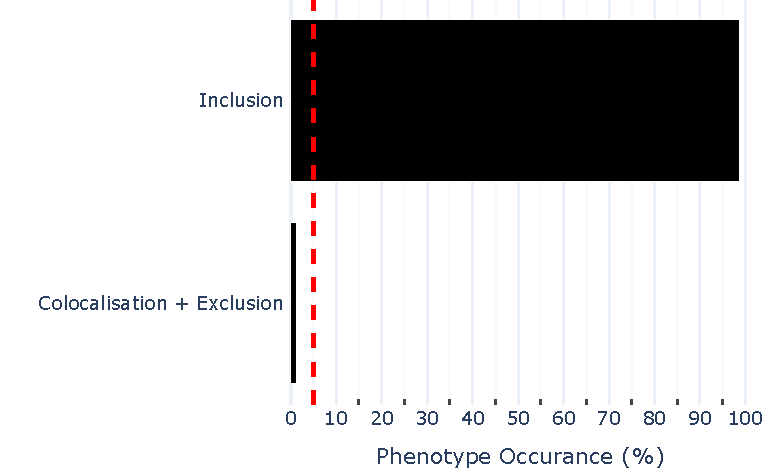
\includegraphics[width=1\linewidth]{09. Chapter 4/Figs/01. pIB/03. IFIT2/02. IFIT2A/01. bar_i2a_293t.pdf}
    \end{subfigure}
    \begin{subfigure}{0.495\textwidth}
        \caption{}
        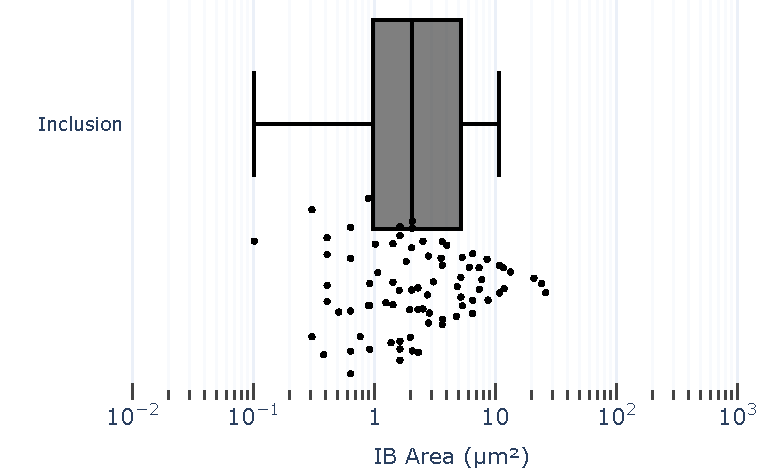
\includegraphics[width=1\linewidth]{09. Chapter 4/Figs/01. pIB/03. IFIT2/02. IFIT2A/02. box_i2a_293t.pdf}
    \end{subfigure}
    \caption[Observed Phenotypes of Nascent Human IFIT2 in the Context of hRSV Pseudo Inclusion Bodies in 293T Cell Line, as Detected by IFIT2(A) Antibody.]{\textbf{Observed Phenotypes of Nascent Human IFIT2 in the Context of hRSV Pseudo Inclusion Bodies in 293T Cell Line, as Detected by IFIT2(A) Antibody.} 293T cells were transfected with hRSV N and P containing plasmids using TransIT-X2 and were fixed after 24 hours. Cells were labeled with anti-RSV N and anti-IFIT2(A) antibodies and imaged on confocal microscope. Panel (a) shows percentual proportions of observed phenotypes between hRSV pseudo inclusion bodies and human IFIT2 (81 observations), with the red dotted line denoting the 5\% threshold, marking phenotypes considered relevant above this limit. Panel (b) shows the IB area in \(\mu \mbox{m}^2\) per observed relevant phenotype.}
    \label{fig:Observed Phenotypes of Nascent Human IFIT2 in the Context of hRSV Pseudo Inclusion Bodies in 293T Cell Line, as Detected by IFIT2(A) Antibody}
\end{figure}

\begin{figure}
    \centering
    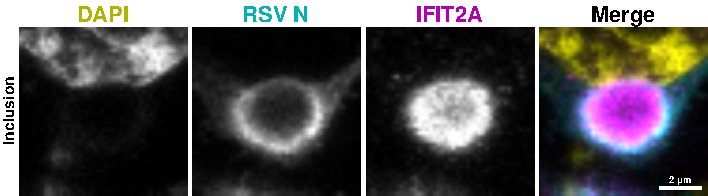
\includegraphics[width=1\linewidth]{09. Chapter 4/Figs/01. pIB/03. IFIT2/02. IFIT2A/03. i2a-293t-hnhp.pdf} 
    \caption[Representative Images of Observed Phenotypes of Nascent Human IFIT2 in the Context of hRSV Pseudo Inclusion Bodies in 293T Cell Line, as Detected by IFIT2(A) Antibody.]{\textbf{Representative Images of Observed Phenotypes of Nascent Human IFIT2 in the Context of hRSV Pseudo Inclusion Bodies in 293T Cell Line, as Detected by IFIT2(A) Antibody.} 293T cells were transfected with hRSV N and P containing plasmids using TransIT-X2 and were fixed after 24 hours. Cellular nuclei were stained with DAPI (yellow), and cells were double-labeled with anti-RSV N (cyan) and anti-IFIT2(A) (magenta) antibodies. This figure showcases representative examples of relevant phenotypes in the interaction between human IFIT2 and hRSV pseudo inclusion bodies. These phenotypes are presented in descending order based on their percentage proportions. The scale bar indicates 2 \(\mu \mbox{m}\).}
    \label{fig:Representative Images of Observed Phenotypes of Nascent Human IFIT2 in the Context of hRSV Pseudo Inclusion Bodies in 293T Cell Line, as Detected by IFIT2(A) Antibody}
\end{figure}

99
2

\begin{figure}
    \begin{subfigure}{0.495\textwidth}
        \caption{}
        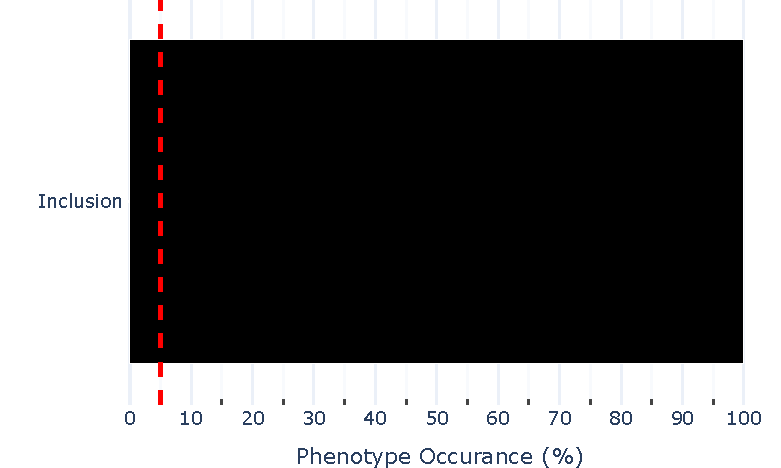
\includegraphics[width=1\linewidth]{09. Chapter 4/Figs/01. pIB/03. IFIT2/02. IFIT2A/04. bar_i2a_vero_hnhp.pdf} 
    \end{subfigure}
    \begin{subfigure}{0.495\textwidth}
        \caption{}
        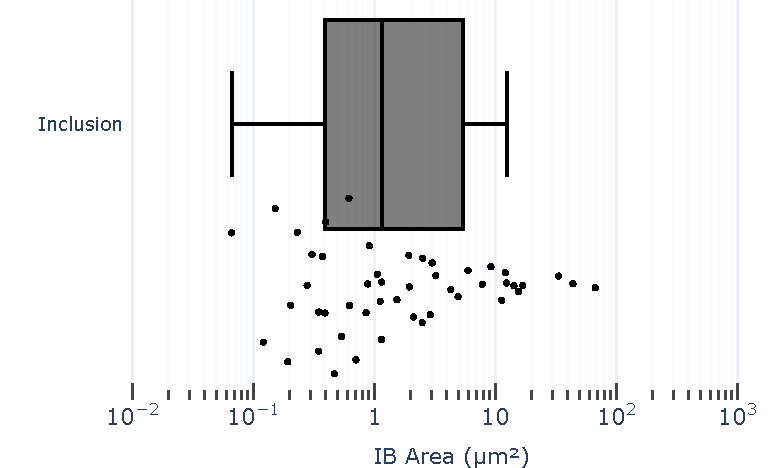
\includegraphics[width=1\linewidth]{09. Chapter 4/Figs/01. pIB/03. IFIT2/02. IFIT2A/05. box_i2a_vero_hnhp.pdf}
    \end{subfigure}
    \caption[Observed Phenotypes of Nascent Monkey IFIT2 in the Context of hRSV Pseudo Inclusion Bodies in Vero Cell Line, as Detected by IFIT2(A) Antibody.]{\textbf{Observed Phenotypes of Nascent Monkey IFIT2 in the Context of hRSV Pseudo Inclusion Bodies in Vero Cell Line, as Detected by IFIT2(A) Antibody.} Vero cells were transfected with hRSV N and P containing plasmids using TransIT-X2 and were fixed after 24 hours. Cells were labeled with anti-RSV N and anti-IFIT2(A) antibodies and imaged on confocal microscope. Panel (a) shows percentual proportions of observed phenotypes between hRSV pseudo inclusion bodies and monkey IFIT2 (48 observations), with the red dotted line denoting the 5\% threshold, marking phenotypes considered relevant above this limit. Panel (b) shows the IB area in \(\mu \mbox{m}^2\) per observed relevant phenotype.}
    \label{fig:Observed Phenotypes of Nascent Monkey IFIT2 in the Context of hRSV Pseudo Inclusion Bodies in Vero Cell Line, as Detected by IFIT2(A) Antibody}
\end{figure}

\begin{figure}
    \centering
    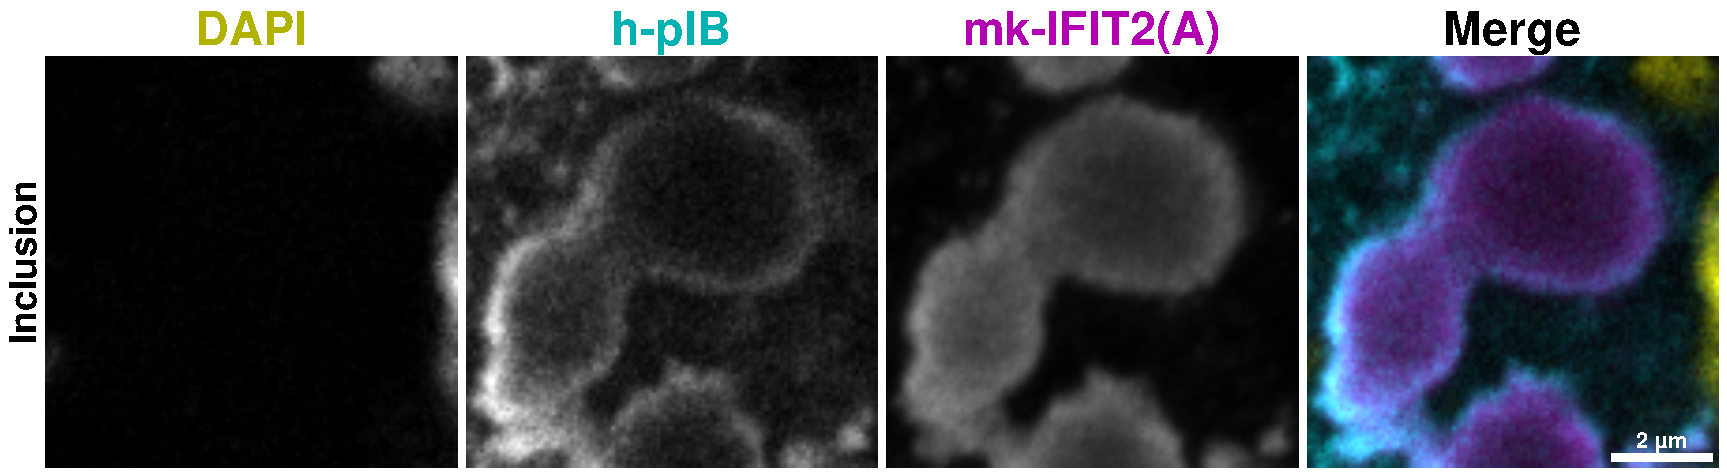
\includegraphics[width=1\linewidth]{09. Chapter 4/Figs/01. pIB/03. IFIT2/02. IFIT2A/06. i2a-vero-hnhp.pdf}  
    \caption[Representative Images of Observed Phenotypes of Nascent Human IFIT2 in the Context of hRSV Pseudo Inclusion Bodies in Vero Cell Line, as Detected by IFIT2(A) Antibody.]{\textbf{Representative Images of Observed Phenotypes of Nascent Human IFIT2 in the Context of hRSV Pseudo Inclusion Bodies in Vero Cell Line, as Detected by IFIT2(A) Antibody.} Vero cells were transfected with hRSV N and P containing plasmids using TransIT-X2 and were fixed after 24 hours. Cellular nuclei were stained with DAPI (yellow), and cells were double-labeled with anti-RSV N (cyan) and anti-IFIT2(A) (magenta) antibodies. This figure showcases representative examples of relevant phenotypes in the interaction between monkey IFIT2 and hRSV pseudo inclusion bodies. These phenotypes are presented in descending order based on their percentage proportions. The scale bar indicates 2 \(\mu \mbox{m}\).}
    \label{fig:Representative Images of Observed Phenotypes of Nascent Human IFIT2 in the Context of hRSV Pseudo Inclusion Bodies in Vero Cell Line, as Detected by IFIT2(A) Antibody}
\end{figure}

100
1.2

\begin{figure}
    \begin{subfigure}{0.495\textwidth}
        \caption{}
        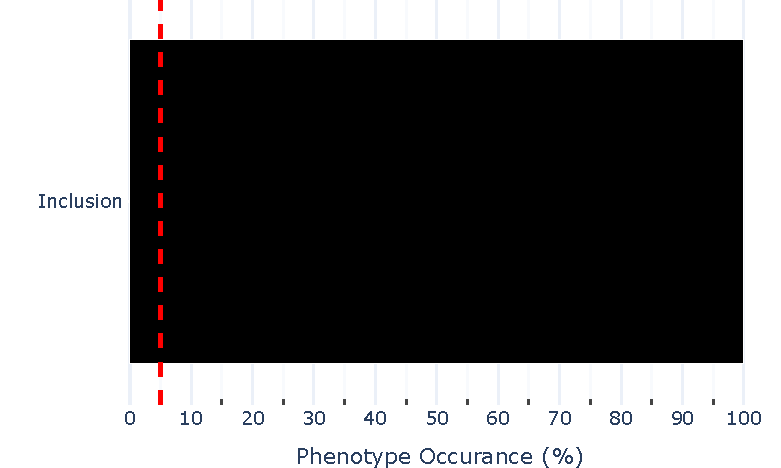
\includegraphics[width=1\linewidth]{09. Chapter 4/Figs/01. pIB/03. IFIT2/02. IFIT2A/07. bar_i2a_vero_bnbp.pdf} 
    \end{subfigure}
    \begin{subfigure}{0.495\textwidth}
        \caption{}
        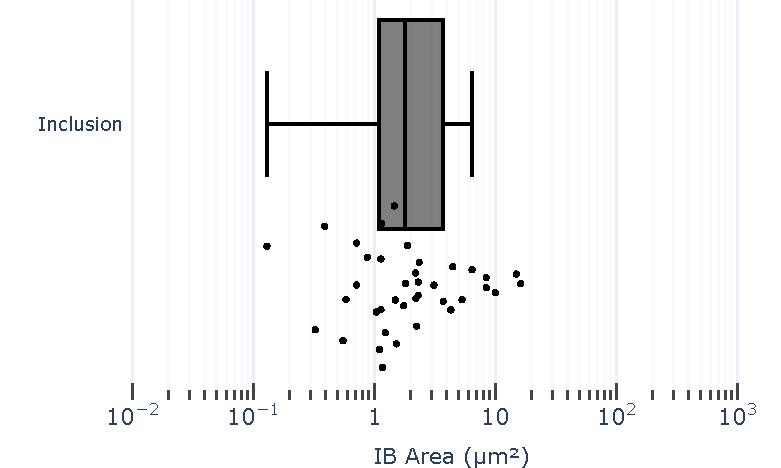
\includegraphics[width=1\linewidth]{09. Chapter 4/Figs/01. pIB/03. IFIT2/02. IFIT2A/08. box_i2a_vero_bnbp.pdf}
    \end{subfigure}
    \caption[Observed Phenotypes of Nascent Monkey IFIT2 in the Context of bRSV Pseudo Inclusion Bodies in Vero Cell Line, as Detected by IFIT2(A) Antibody.]{\textbf{Observed Phenotypes of Nascent Monkey IFIT2 in the Context of bRSV Pseudo Inclusion Bodies in Vero Cell Line, as Detected by IFIT2(A) Antibody.} Vero cells were transfected with bRSV N and P containing plasmids using TransIT-X2 and were fixed after 24 hours. Cells were labeled with anti-RSV N and anti-IFIT2(A) antibodies and imaged on confocal microscope. Panel (a) shows percentual proportions of observed phenotypes between bRSV pseudo inclusion bodies and monkey IFIT2 (38 observations), with the red dotted line denoting the 5\% threshold, marking phenotypes considered relevant above this limit. Panel (b) shows the IB area in \(\mu \mbox{m}^2\) per observed relevant phenotype.}
    \label{fig:Observed Phenotypes of Nascent Monkey IFIT2 in the Context of bRSV Pseudo Inclusion Bodies in Vero Cell Line, as Detected by IFIT2(A) Antibody}
\end{figure}

\begin{figure}
    \centering
    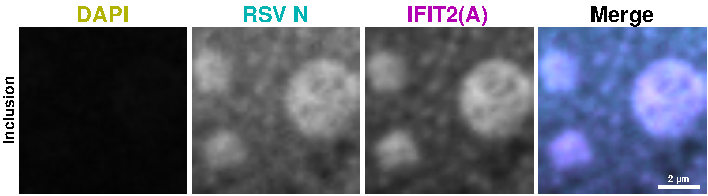
\includegraphics[width=1\linewidth]{09. Chapter 4/Figs/01. pIB/03. IFIT2/02. IFIT2A/09. i2a-vero-bnbp.pdf} 
    \caption[Representative Images of Observed Phenotypes of Nascent Human IFIT2 in the Context of bRSV Pseudo Inclusion Bodies in Vero Cell Line, as Detected by IFIT2(A) Antibody.]{\textbf{Representative Images of Observed Phenotypes of Nascent Human IFIT2 in the Context of bRSV Pseudo Inclusion Bodies in Vero Cell Line, as Detected by IFIT2(A) Antibody.} Vero cells were transfected with bRSV N and P containing plasmids using TransIT-X2 and were fixed after 24 hours. Cellular nuclei were stained with DAPI (yellow), and cells were double-labeled with anti-RSV N (cyan) and anti-IFIT2(A) (magenta) antibodies. This figure showcases representative examples of relevant phenotypes in the interaction between monkey IFIT2 and bRSV pseudo inclusion bodies. These phenotypes are presented in descending order based on their percentage proportions. The scale bar indicates 2 \(\mu \mbox{m}\).}
    \label{fig:Representative Images of Observed Phenotypes of Nascent Human IFIT2 in the Context of bRSV Pseudo Inclusion Bodies in Vero Cell Line, as Detected by IFIT2(A) Antibody}
\end{figure}

100
1.8

\begin{figure}
    \begin{subfigure}{0.495\textwidth}
        \caption{}
        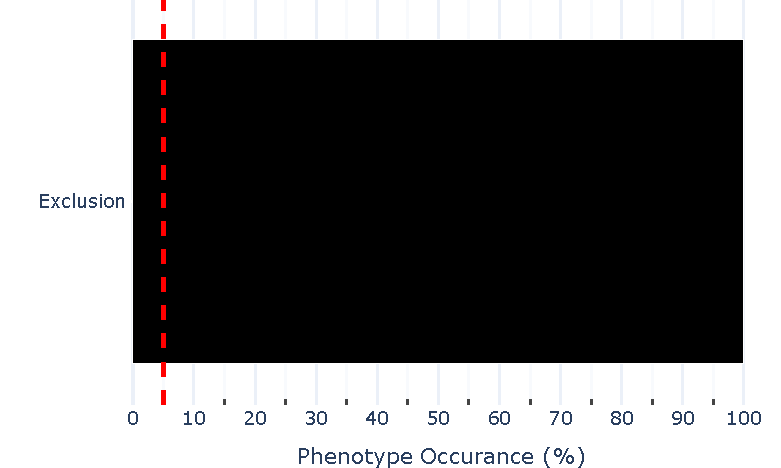
\includegraphics[width=1\linewidth]{09. Chapter 4/Figs/01. pIB/03. IFIT2/03. IFIT2B/01. bar_i2b_293t.pdf} 
    \end{subfigure}
    \begin{subfigure}{0.495\textwidth}
        \caption{}
        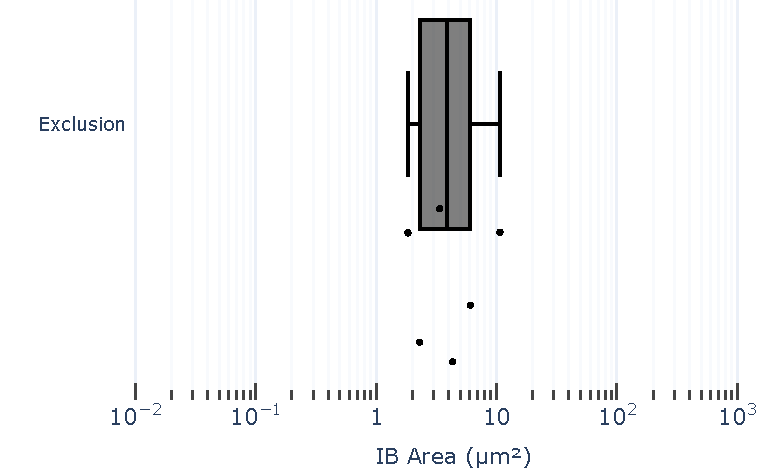
\includegraphics[width=1\linewidth]{09. Chapter 4/Figs/01. pIB/03. IFIT2/03. IFIT2B/02. box_i2b_293t.pdf}
    \end{subfigure}
    \caption[Observed Phenotypes of Nascent Human IFIT2 in the Context of hRSV Pseudo Inclusion Bodies in 293T Cell Line, as Detected by IFIT2(B) Antibody.]{\textbf{Observed Phenotypes of Nascent Human IFIT2 in the Context of hRSV Pseudo Inclusion Bodies in 293T Cell Line, as Detected by IFIT2(B) Antibody.} 293T cells were transfected with hRSV N and P containing plasmids using TransIT-X2 and were fixed after 24 hours. Cells were labeled with anti-RSV N and anti-IFIT2(B) antibodies and imaged on confocal microscope. Panel (a) shows percentual proportions of observed phenotypes between hRSV pseudo inclusion bodies and human IFIT2 (6 observations), with the red dotted line denoting the 5\% threshold, marking phenotypes considered relevant above this limit. Panel (b) shows the IB area in \(\mu \mbox{m}^2\) per observed relevant phenotype.}
    \label{fig:Observed Phenotypes of Nascent Human IFIT2 in the Context of hRSV Pseudo Inclusion Bodies in 293T Cell Line, as Detected by IFIT2(B) Antibody}
\end{figure}

\begin{figure}
    \centering
    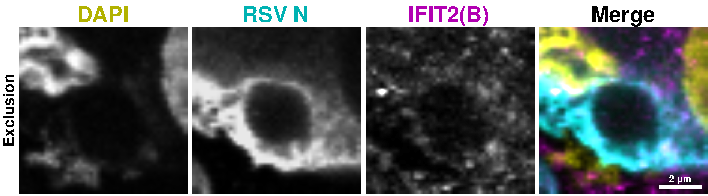
\includegraphics[width=1\linewidth]{09. Chapter 4/Figs/01. pIB/03. IFIT2/03. IFIT2B/03. i2b-293t-hnhp.pdf} 
    \caption[Representative Images of Observed Phenotypes of Nascent Human IFIT2 in the Context of hRSV Pseudo Inclusion Bodies in 293T Cell Line, as Detected by IFIT2(B) Antibody.]{\textbf{Representative Images of Observed Phenotypes of Nascent Human IFIT2 in the Context of hRSV Pseudo Inclusion Bodies in 293T Cell Line, as Detected by IFIT2(B) Antibody.} 293T cells were transfected with hRSV N and P containing plasmids using TransIT-X2 and were fixed after 24 hours. Cellular nuclei were stained with DAPI (yellow), and cells were double-labeled with anti-RSV N (cyan) and anti-IFIT2(B) (magenta) antibodies. This figure showcases representative examples of relevant phenotypes in the interaction between human IFIT2 and hRSV pseudo inclusion bodies. These phenotypes are presented in descending order based on their percentage proportions. The scale bar indicates 2 \(\mu \mbox{m}\).}
    \label{fig:Representative Images of Observed Phenotypes of Nascent Human IFIT2 in the Context of hRSV Pseudo Inclusion Bodies in 293T Cell Line, as Detected by IFIT2(B) Antibody}
\end{figure}

100
4

\begin{figure}
    \begin{subfigure}{0.495\textwidth}
        \caption{}
        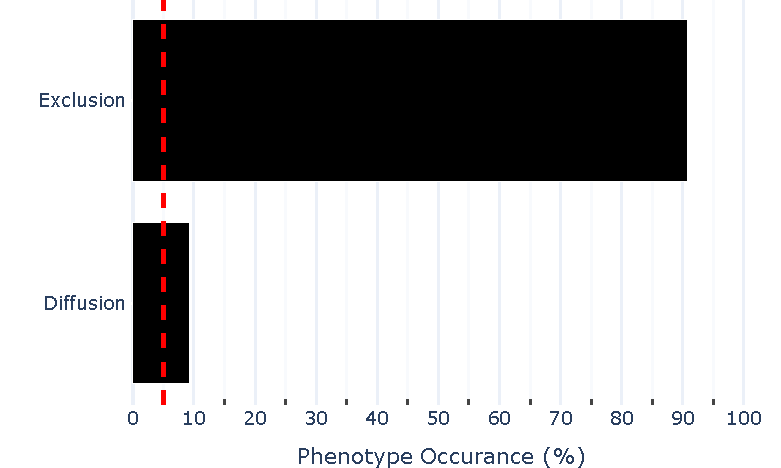
\includegraphics[width=1\linewidth]{09. Chapter 4/Figs/01. pIB/03. IFIT2/03. IFIT2B/04. bar_i2b_vero_hnhp.pdf} 
    \end{subfigure}
    \begin{subfigure}{0.495\textwidth}
        \caption{}
        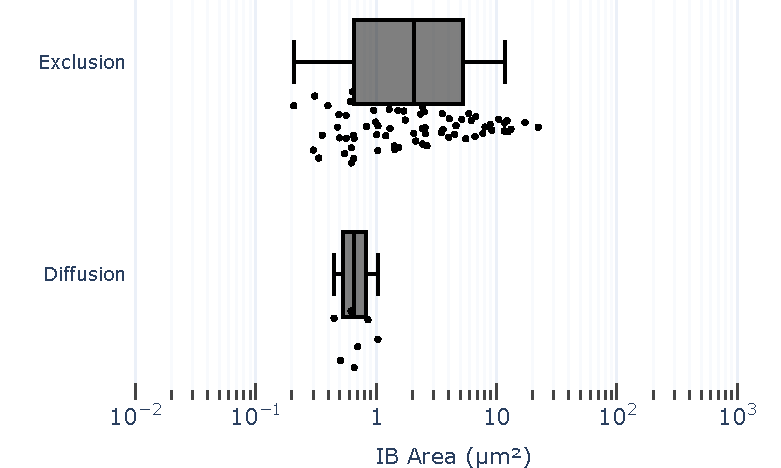
\includegraphics[width=1\linewidth]{09. Chapter 4/Figs/01. pIB/03. IFIT2/03. IFIT2B/05. box_i2b_vero_hnhp.pdf}
    \end{subfigure}
    \caption[Observed Phenotypes of Nascent Monkey IFIT2 in the Context of hRSV Pseudo Inclusion Bodies in Vero Cell Line, as Detected by IFIT2(B) Antibody.]{\textbf{Observed Phenotypes of Nascent Monkey IFIT2 in the Context of hRSV Pseudo Inclusion Bodies in Vero Cell Line, as Detected by IFIT2(B) Antibody.} Vero cells were transfected with hRSV N and P containing plasmids using TransIT-X2 and were fixed after 24 hours. Cells were labeled with anti-RSV N and anti-IFIT2(B) antibodies and imaged on confocal microscope. Panel (a) shows percentual proportions of observed phenotypes between hRSV pseudo inclusion bodies and monkey IFIT2 (76 observations), with the red dotted line denoting the 5\% threshold, marking phenotypes considered relevant above this limit. Panel (b) shows the IB area in \(\mu \mbox{m}^2\) per observed relevant phenotype.}
    \label{fig:Observed Phenotypes of Nascent Monkey IFIT2 in the Context of hRSV Pseudo Inclusion Bodies in Vero Cell Line, as Detected by IFIT2(B) Antibody}
\end{figure}

\begin{figure}
    \centering
    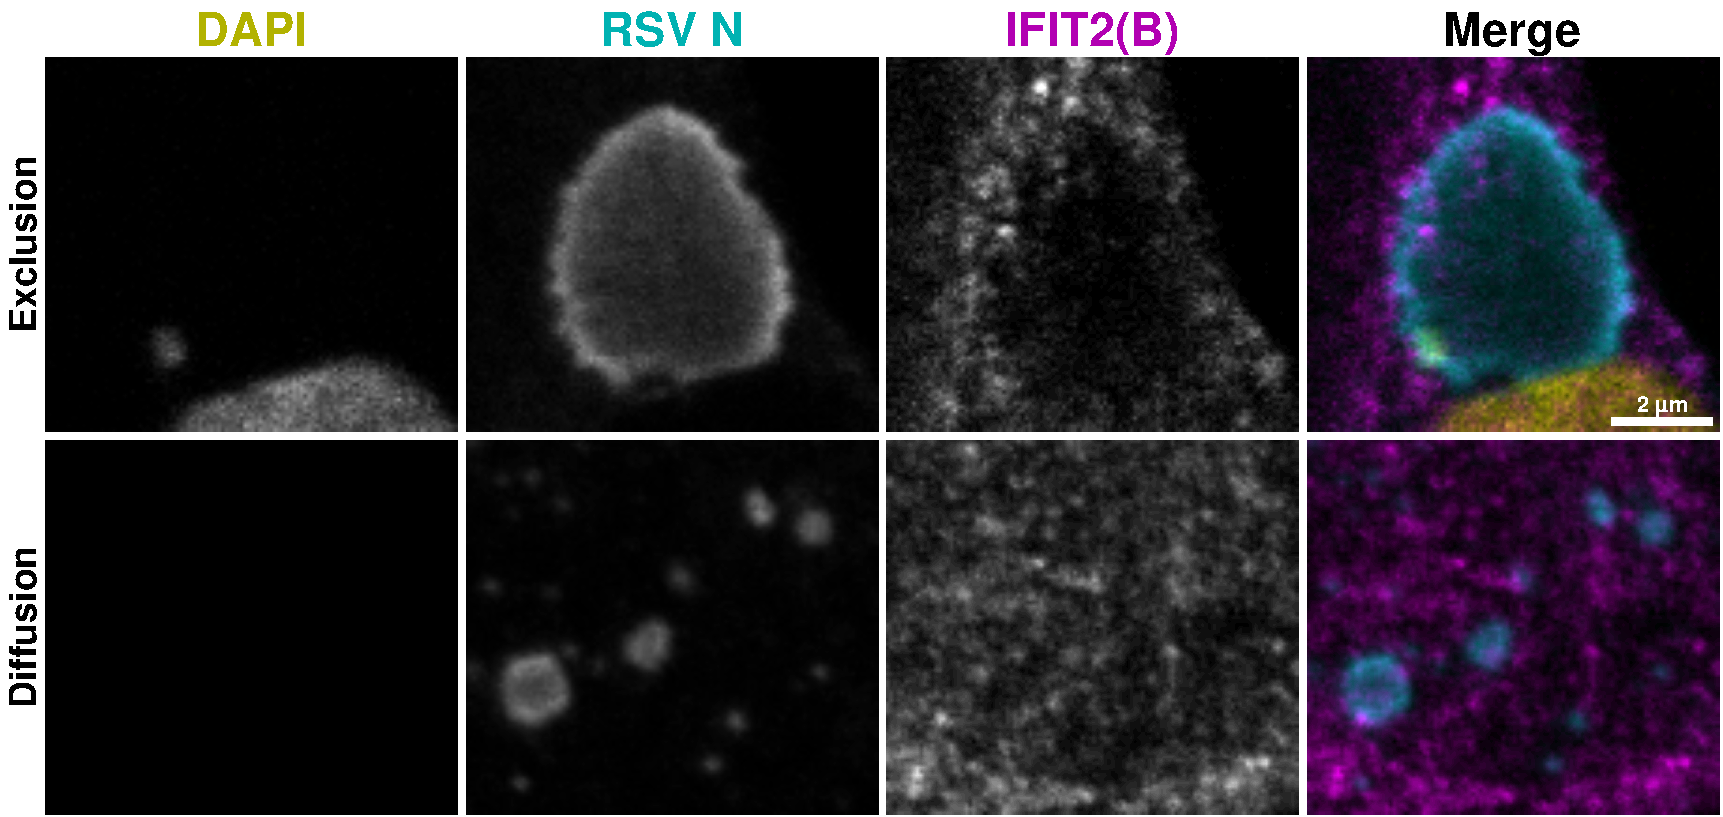
\includegraphics[width=1\linewidth]{09. Chapter 4/Figs/01. pIB/03. IFIT2/03. IFIT2B/06. i2b-vero-hnhp.pdf} 
    \caption[Representative Images of Observed Phenotypes of Nascent Human IFIT2 in the Context of hRSV Pseudo Inclusion Bodies in Vero Cell Line, as Detected by IFIT2(B) Antibody.]{\textbf{Representative Images of Observed Phenotypes of Nascent Human IFIT2 in the Context of hRSV Pseudo Inclusion Bodies in Vero Cell Line, as Detected by IFIT2(B) Antibody.} Vero cells were transfected with hRSV N and P containing plasmids using TransIT-X2 and were fixed after 24 hours. Cellular nuclei were stained with DAPI (yellow), and cells were double-labeled with anti-RSV N (cyan) and anti-IFIT2(B) (magenta) antibodies. This figure showcases representative examples of relevant phenotypes in the interaction between monkey IFIT2 and hRSV pseudo inclusion bodies. These phenotypes are presented in descending order based on their percentage proportions. The scale bar indicates 2 \(\mu \mbox{m}\).}
    \label{fig:Representative Images of Observed Phenotypes of Nascent Human IFIT2 in the Context of hRSV Pseudo Inclusion Bodies in Vero Cell Line, as Detected by IFIT2(B) Antibody}
\end{figure}

91 9
2 0.63

% summary
Both endogenous human and monkey IFIT2 forms inclusions inside human RSV pseudo-IBs. Monkey IFIT2 also colocalises to the pIB filamentous network (this structure was not observed in the human experiment). The identical staining can be observed in monkey cells with overexpressed human IFIT2-FLAG.

Endogenous monkey IFIT2 is excluded from human pIB and the pIB associated filamentous network. Overexpressed human IFIT2-FLAG is detected by the antibody and shows inclusions inside the human pIB structures, which is consistent to data from IFIT2(A) staining and FLAG staining of IFIT2-FLAG overexpressed samples. Interestingly, IFIT2(B) antibody shows exclusion from the pIB filamentous network, which was colocalised by IFIT2(A) and FLAG antibodies.

% exogenous
Monkey cells transfected with human RSV N and P, along with human IFIT2-FLAG show concentration within the pIB structures as well as the pIB filamentous network. In this experiment we are detecting both human and monkey IFIT2, however we can see a huge difference in IFIT2 expression between some cells (bottom panel; cells in the periphery of the picture), suggesting that what we are mainly detecting is the overexpressed human IFIT2-FLAG.

\begin{figure}
    \begin{subfigure}{0.495\textwidth}
        \caption{}
        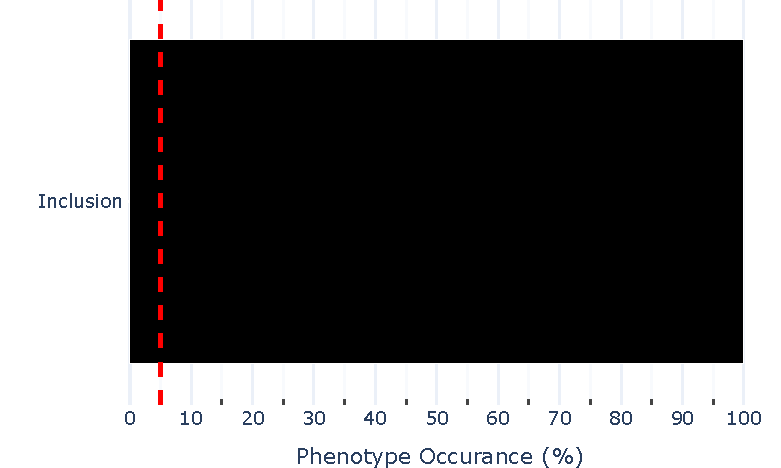
\includegraphics[width=1\linewidth]{09. Chapter 4/Figs/01. pIB/03. IFIT2/04. IFIT2-FLAG/01. IFIT2A/01. bar_i2a_hnhp.pdf} 
    \end{subfigure}
    \begin{subfigure}{0.495\textwidth}
        \caption{}
        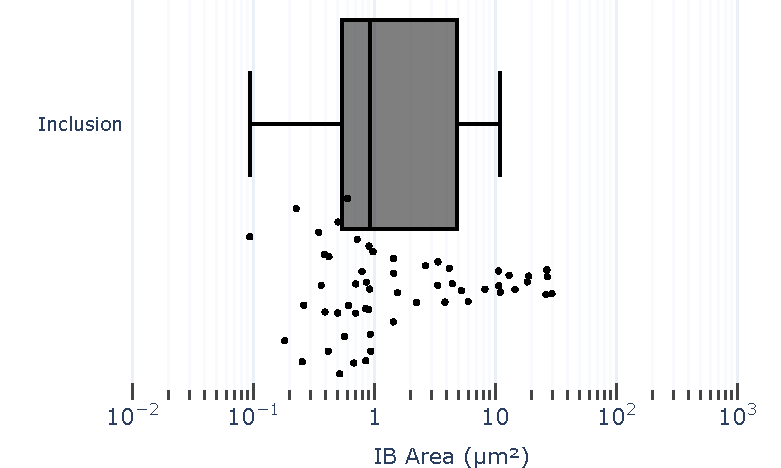
\includegraphics[width=1\linewidth]{09. Chapter 4/Figs/01. pIB/03. IFIT2/04. IFIT2-FLAG/01. IFIT2A/02. box_i2a_hnhp.pdf}
    \end{subfigure}
    \caption[Observed Phenotypes of Exogenous Human IFIT2 in the Context of hRSV Pseudo Inclusion Bodies in Vero Cell Line, as Detected by IFIT2(A) Antibody.]{\textbf{Observed Phenotypes of Exogenous Human IFIT2 in the Context of hRSV Pseudo Inclusion Bodies in Vero Cell Line, as Detected by IFIT2(A) Antibody.} Vero cells were transfected with hRSV N and P, along with human IFIT2-FLAG containing plasmids using TransIT-X2 and were fixed after 24 hours. Cells were labeled with anti-RSV N and anti-IFIT2(A) antibodies and imaged on confocal microscope. Panel (a) shows percentual proportions of observed phenotypes between hRSV pseudo inclusion bodies and exogenous human IFIT2 (56 observations), with the red dotted line denoting the 5\% threshold, marking phenotypes considered relevant above this limit. Panel (b) shows the IB area in \(\mu \mbox{m}^2\) per observed relevant phenotype.}
    \label{fig:Observed Phenotypes of Exogenous Human IFIT2 in the Context of hRSV Pseudo Inclusion Bodies in Vero Cell Line, as Detected by IFIT2(A) Antibody}
\end{figure}

\begin{figure}
    \centering
    \includegraphics[width=1\linewidth]{09. Chapter 4/Figs/01. pIB/03. IFIT2/04. IFIT2-FLAG/01. IFIT2A/03. i2a-hi2f-hnhp.pdf}
    \caption[Representative Images of Observed Phenotypes of Exogenous Human IFIT2 in the Context of hRSV Pseudo Inclusion Bodies in Vero Cell Line, as Detected by IFIT2(A) Antibody.]{\textbf{Representative Images of Observed Phenotypes of Exogenous Human IFIT2 in the Context of hRSV Pseudo Inclusion Bodies in Vero Cell Line, as Detected by IFIT2(A) Antibody.} Vero cells were transfected with hRSV N and P, along with human IFIT2-FLAG containing plasmids using TransIT-X2 and were fixed after 24 hours. Cellular nuclei were stained with DAPI (yellow), and cells were double-labeled with anti-RSV N (cyan) and anti-IFIT2(A) (magenta) antibodies. This figure showcases representative examples of relevant phenotypes in the interaction between exogenous human IFIT2 and hRSV pseudo inclusion bodies. These phenotypes are presented in descending order based on their percentage proportions. The scale bar indicates 2 \(\mu \mbox{m}\).}
    \label{fig:Representative Images of Observed Phenotypes of Exogenous Human IFIT2 in the Context of hRSV Pseudo Inclusion Bodies in Vero Cell Line, as Detected by IFIT2(A) Antibody}
\end{figure}

100
0.9

Monkey cells transfected with human RSV N and P, along with human IFIT2-FLAG show concentration within the pIB structures but show exclusion from the pIB filamentous network (or partial colocalsiation?). This suggest that the IFIT2(B) antibody can indeed detect IFIT2 but the overexpressed IFIT2 observed between the inclusion and the one interacting with the filamentous network is somehow different (epitope masking?).

\begin{figure}
    \begin{subfigure}{0.495\textwidth}
        \caption{}
        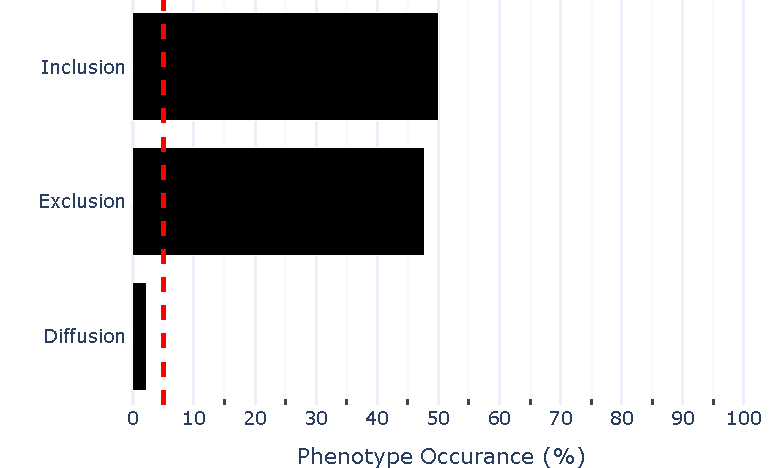
\includegraphics[width=1\linewidth]{09. Chapter 4/Figs/01. pIB/03. IFIT2/04. IFIT2-FLAG/02. IFIT2B/01. bar_i2b_hnhp.pdf}
    \end{subfigure}
    \begin{subfigure}{0.495\textwidth}
        \caption{}
        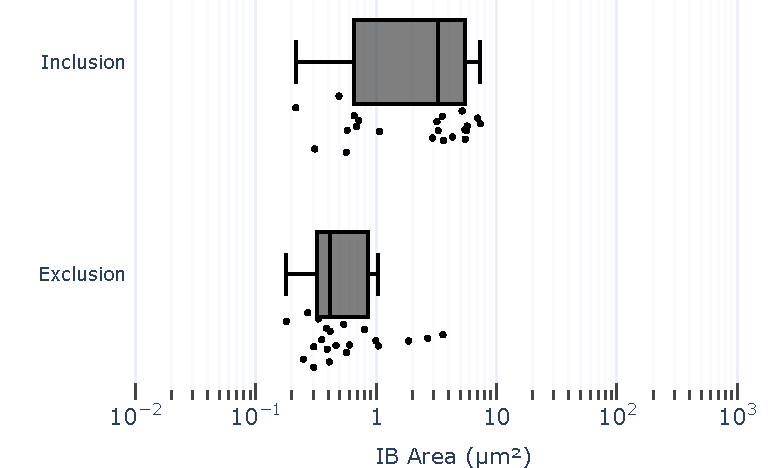
\includegraphics[width=1\linewidth]{09. Chapter 4/Figs/01. pIB/03. IFIT2/04. IFIT2-FLAG/02. IFIT2B/02. box_i2a_hnhp.pdf}
    \end{subfigure}
    \caption[Observed Phenotypes of Exogenous Human IFIT2 in the Context of hRSV Pseudo Inclusion Bodies in Vero Cell Line, as Detected by IFIT2(B) Antibody.]{\textbf{Observed Phenotypes of Exogenous Human IFIT2 in the Context of hRSV Pseudo Inclusion Bodies in Vero Cell Line, as Detected by IFIT2(B) Antibody.} Vero cells were transfected with hRSV N and P, along with human IFIT2-FLAG containing plasmids using TransIT-X2 and were fixed after 24 hours. Cells were labeled with anti-RSV N and anti-IFIT2(B) antibodies and imaged on confocal microscope. Panel (a) shows percentual proportions of observed phenotypes between hRSV pseudo inclusion bodies and exogenous human IFIT2 (44 observations), with the red dotted line denoting the 5\% threshold, marking phenotypes considered relevant above this limit. Panel (b) shows the IB area in \(\mu \mbox{m}^2\) per observed relevant phenotype.}
    \label{fig:Observed Phenotypes of Exogenous Human IFIT2 in the Context of hRSV Pseudo Inclusion Bodies in Vero Cell Line, as Detected by IFIT2(B) Antibody}
\end{figure}

\begin{figure}
    \centering
    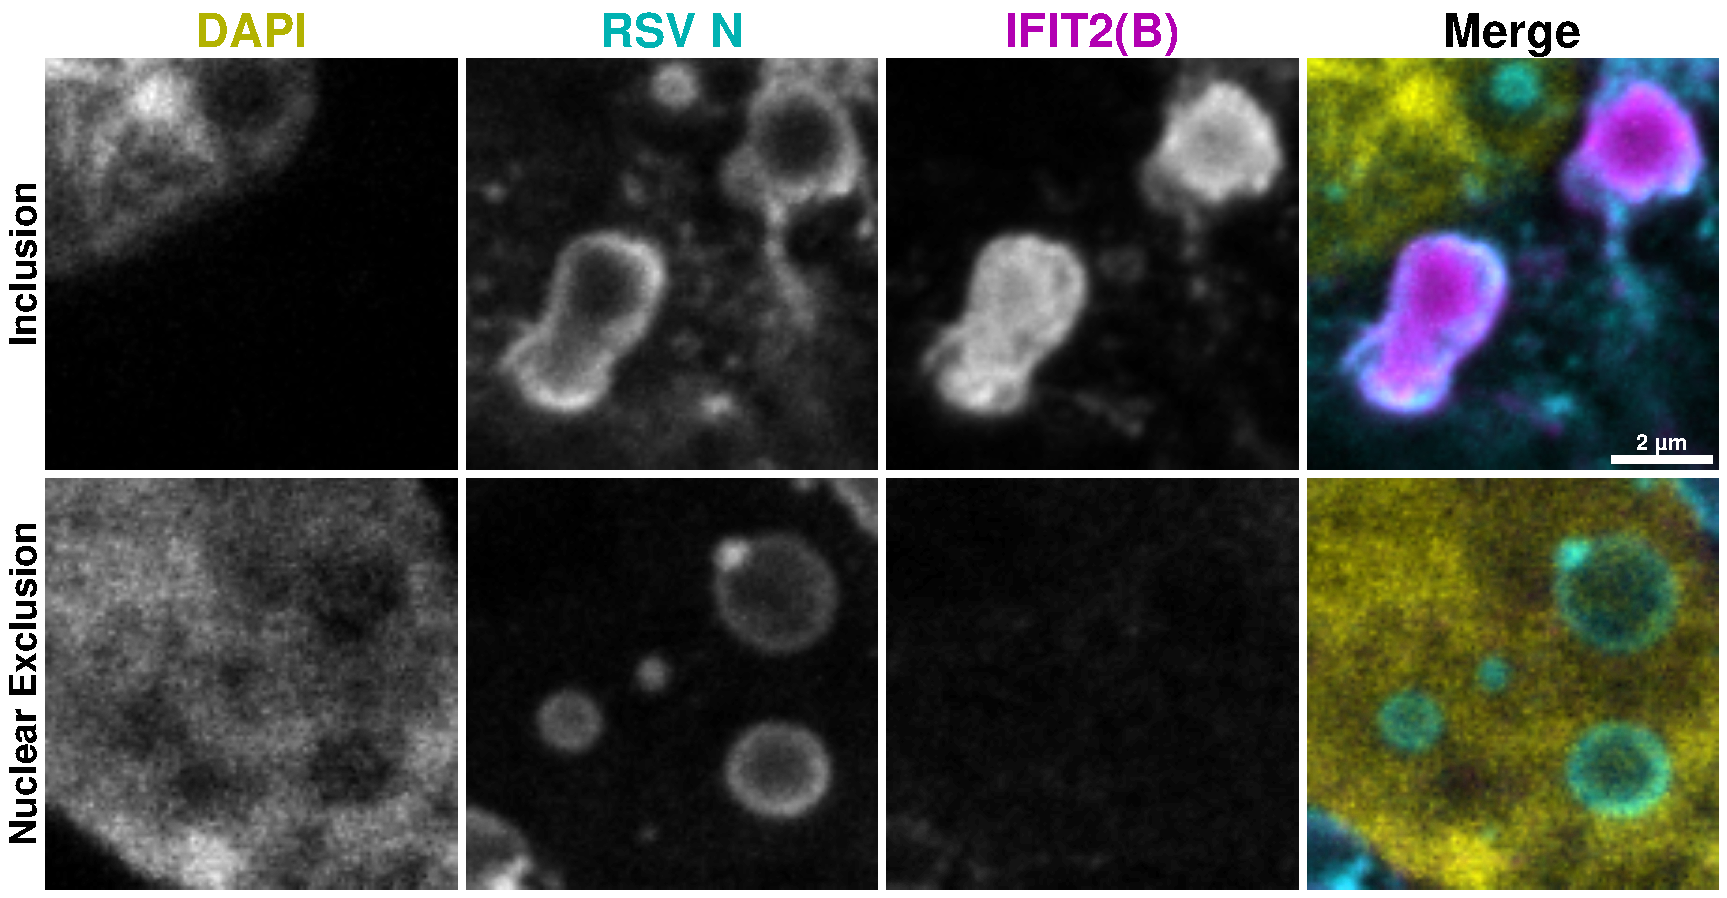
\includegraphics[width=1\linewidth]{09. Chapter 4/Figs/01. pIB/03. IFIT2/04. IFIT2-FLAG/02. IFIT2B/03. i2b-hi2f-hnhp.pdf}
    \caption[Representative Images of Observed Phenotypes of Exogenous Human IFIT2 in the Context of hRSV Pseudo Inclusion Bodies in Vero Cell Line, as Detected by IFIT2(B) Antibody.]{\textbf{Representative Images of Observed Phenotypes of Exogenous Human IFIT2 in the Context of hRSV Pseudo Inclusion Bodies in Vero Cell Line, as Detected by IFIT2(B) Antibody.} Vero cells were transfected with hRSV N and P, along with human IFIT2-FLAG containing plasmids using TransIT-X2 and were fixed after 24 hours. Cellular nuclei were stained with DAPI (yellow), and cells were double-labeled with anti-RSV N (cyan) and anti-IFIT2(B) (magenta) antibodies. This figure showcases representative examples of relevant phenotypes in the interaction between exogenous human IFIT2 and hRSV pseudo inclusion bodies. These phenotypes are presented in descending order based on their percentage proportions. The scale bar indicates 2 \(\mu \mbox{m}\).}
    \label{fig:Representative Images of Observed Phenotypes of Exogenous Human IFIT2 in the Context of hRSV Pseudo Inclusion Bodies in Vero Cell Line, as Detected by IFIT2(B) Antibody}
\end{figure}

50 47
3.2 0.4

Exogenously expressed human IFIT2 colocalises with the pIB associated filamentous net (top panel). It also forms inclusion inside the human pIB structures. This data is consistent with what we observed with IFIT2(A) antibody. IFIT2 also seems to occasionally form aggregates/spots (highlighted by arrows). These could be functional or just aggregates caused by overexpression, we do not know.

\begin{figure}
    \begin{subfigure}{0.495\textwidth}
        \caption{}
        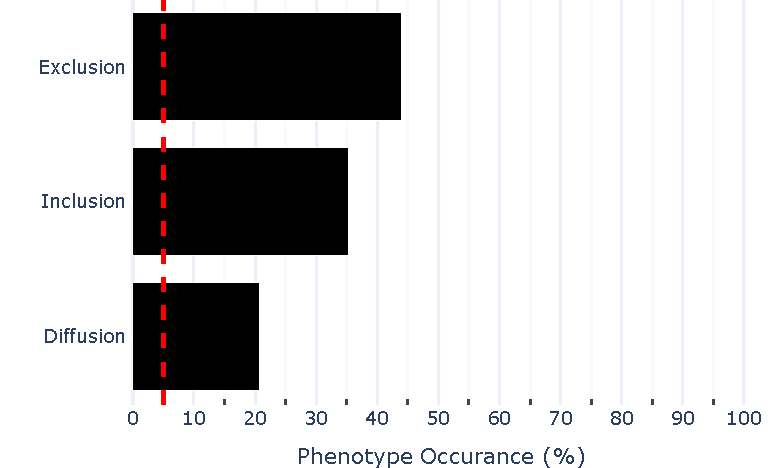
\includegraphics[width=1\linewidth]{09. Chapter 4/Figs/01. pIB/03. IFIT2/04. IFIT2-FLAG/03. FLAG/01. bar_hi2f_hnhp.pdf}
    \end{subfigure}
    \begin{subfigure}{0.495\textwidth}
        \caption{}
        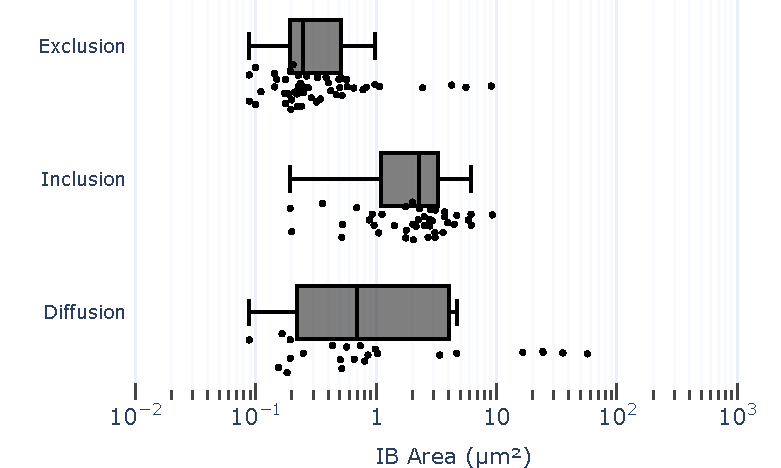
\includegraphics[width=1\linewidth]{09. Chapter 4/Figs/01. pIB/03. IFIT2/04. IFIT2-FLAG/03. FLAG/02. box_hi2f_hnhp.pdf}
    \end{subfigure}
    \caption[Observed Phenotypes of Exogenous Human IFIT2 in the Context of hRSV Pseudo Inclusion Bodies in Vero Cell Line, as Detected by FLAG Antibody.]{\textbf{Observed Phenotypes of Exogenous Human IFIT2 in the Context of hRSV Pseudo Inclusion Bodies in Vero Cell Line, as Detected by FLAG Antibody.} Vero cells were transfected with hRSV N and P, along with human IFIT2-FLAG containing plasmids using TransIT-X2 and were fixed after 24 hours. Cells were labeled with anti-RSV N and anti-FLAG antibodies and imaged on confocal microscope. Panel (a) shows percentual proportions of observed phenotypes between hRSV pseudo inclusion bodies and exogenous human IFIT2 (116 observations), with the red dotted line denoting the 5\% threshold, marking phenotypes considered relevant above this limit. Panel (b) shows the IB area in \(\mu \mbox{m}^2\) per observed relevant phenotype.}
    \label{fig:Observed Phenotypes of Exogenous Human IFIT2 in the Context of hRSV Pseudo Inclusion Bodies in Vero Cell Line, as Detected by FLAG Antibody}
\end{figure}

\begin{figure}
    \centering
    \includegraphics[width=1\linewidth]{09. Chapter 4/Figs/01. pIB/03. IFIT2/04. IFIT2-FLAG/03. FLAG/03. hi2f-hnhp.pdf}
    \caption[Representative Images of Observed Phenotypes of Exogenous Human IFIT2 in the Context of hRSV Pseudo Inclusion Bodies in Vero Cell Line, as Detected by FLAG Antibody.]{\textbf{Representative Images of Observed Phenotypes of Exogenous Human IFIT2 in the Context of hRSV Pseudo Inclusion Bodies in Vero Cell Line, as Detected by FLAG Antibody.} Vero cells were transfected with hRSV N and P, along with human IFIT2-FLAG containing plasmids using TransIT-X2 and were fixed after 24 hours. Cellular nuclei were stained with DAPI (yellow), and cells were double-labeled with anti-RSV N (cyan) and anti-FLAG (magenta) antibodies. This figure showcases representative examples of relevant phenotypes in the interaction between exogenous human IFIT2 and hRSV pseudo inclusion bodies. These phenotypes are presented in descending order based on their percentage proportions. The scale bar indicates 2 \(\mu \mbox{m}\).}
    \label{fig:Representative Images of Observed Phenotypes of Exogenous Human IFIT2 in the Context of hRSV Pseudo Inclusion Bodies in Vero Cell Line, as Detected by FLAG Antibody}
\end{figure}

49 35 21
0.23 2.1 0.7

Exogenous bovine IFIT2 colocalises with the edge of human pIB structures. This is unusual as human IFIT2 data suggest inclusions with regards to pIBs.  

\begin{figure}
    \begin{subfigure}{0.495\textwidth}
        \caption{}
        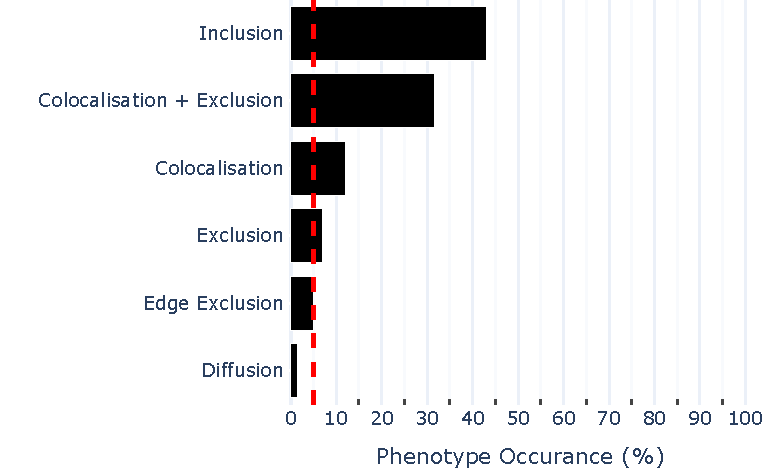
\includegraphics[width=1\linewidth]{09. Chapter 4/Figs/01. pIB/03. IFIT2/04. IFIT2-FLAG/03. FLAG/04. bar_bi2f_hnhp.pdf} 
    \end{subfigure}
    \begin{subfigure}{0.495\textwidth}
        \caption{}
        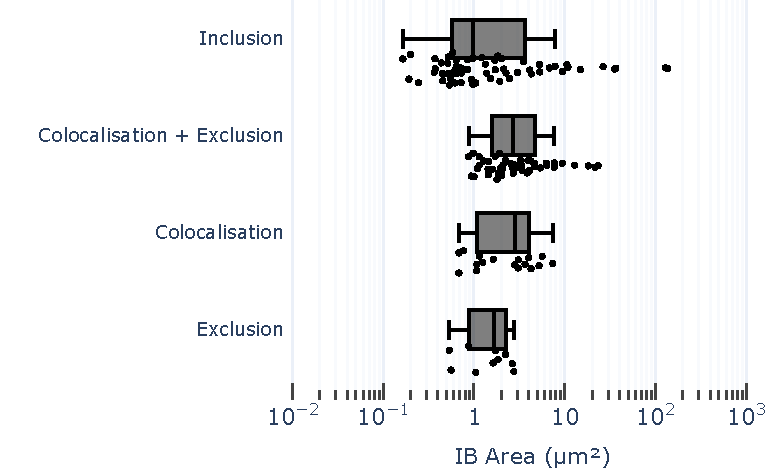
\includegraphics[width=1\linewidth]{09. Chapter 4/Figs/01. pIB/03. IFIT2/04. IFIT2-FLAG/03. FLAG/05. box_bi2f_hnhp.pdf}
    \end{subfigure}
    \caption[Observed Phenotypes of Exogenous Bovine IFIT2 in the Context of hRSV Pseudo Inclusion Bodies in Vero Cell Line, as Detected by FLAG Antibody.]{\textbf{Observed Phenotypes of Exogenous Bovine IFIT2 in the Context of hRSV Pseudo Inclusion Bodies in Vero Cell Line, as Detected by FLAG Antibody.} Vero cells were transfected with hRSV N and P, along with bovine IFIT2-FLAG containing plasmids using TransIT-X2 and were fixed after 24 hours. Cells were labeled with anti-RSV N and anti-FLAG antibodies and imaged on confocal microscope. Panel (a) shows percentual proportions of observed phenotypes between hRSV pseudo inclusion bodies and exogenous bovine IFIT2 (142 observations), with the red dotted line denoting the 5\% threshold, marking phenotypes considered relevant above this limit. Panel (b) shows the IB area in \(\mu \mbox{m}^2\) per observed relevant phenotype.}
    \label{fig:Observed Phenotypes of Exogenous Bovine IFIT2 in the Context of hRSV Pseudo Inclusion Bodies in Vero Cell Line, as Detected by FLAG Antibody}
\end{figure}

\begin{figure}
    \centering
    \includegraphics[width=1\linewidth]{09. Chapter 4/Figs/01. pIB/03. IFIT2/04. IFIT2-FLAG/03. FLAG/06. bi2f-hnhp.pdf}
    \caption[Representative Images of Observed Phenotypes of Exogenous Bovine IFIT2 in the Context of hRSV Pseudo Inclusion Bodies in Vero Cell Line, as Detected by FLAG Antibody.]{\textbf{Representative Images of Observed Phenotypes of Exogenous Bovine IFIT2 in the Context of hRSV Pseudo Inclusion Bodies in Vero Cell Line, as Detected by FLAG Antibody.} Vero cells were transfected with hRSV N and P, along with bovine IFIT2-FLAG containing plasmids using TransIT-X2 and were fixed after 24 hours. Cellular nuclei were stained with DAPI (yellow), and cells were double-labeled with anti-RSV N (cyan) and anti-FLAG (magenta) antibodies. This figure showcases representative examples of relevant phenotypes in the interaction between exogenous bovine IFIT2 and hRSV pseudo inclusion bodies. These phenotypes are presented in descending order based on their percentage proportions. The scale bar indicates 2 \(\mu \mbox{m}\).}
    \label{fig:Representative Images of Observed Phenotypes of Exogenous Bovine IFIT2 in the Context of hRSV Pseudo Inclusion Bodies in Vero Cell Line, as Detected by FLAG Antibody}
\end{figure}

46 31 12 6
1 2.8 2.8 1.7

\begin{figure}
    \begin{subfigure}{0.495\textwidth}
        \caption{}
        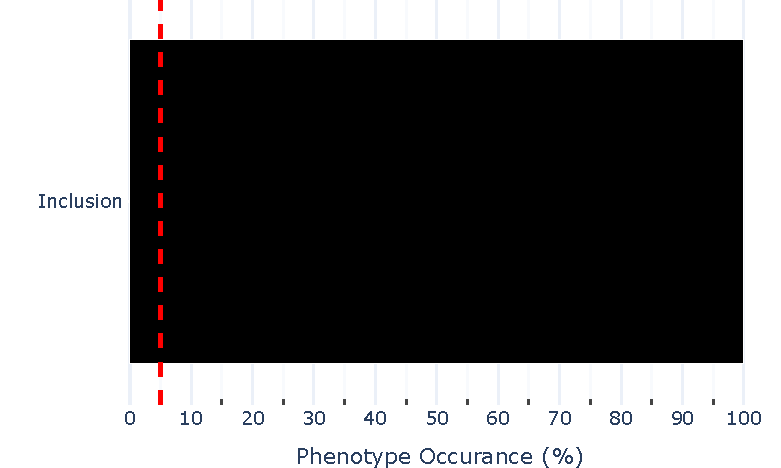
\includegraphics[width=1\linewidth]{09. Chapter 4/Figs/01. pIB/03. IFIT2/04. IFIT2-FLAG/03. FLAG/07. bar_bi2f_bnbp.pdf} 
    \end{subfigure}
    \begin{subfigure}{0.495\textwidth}
        \caption{}
        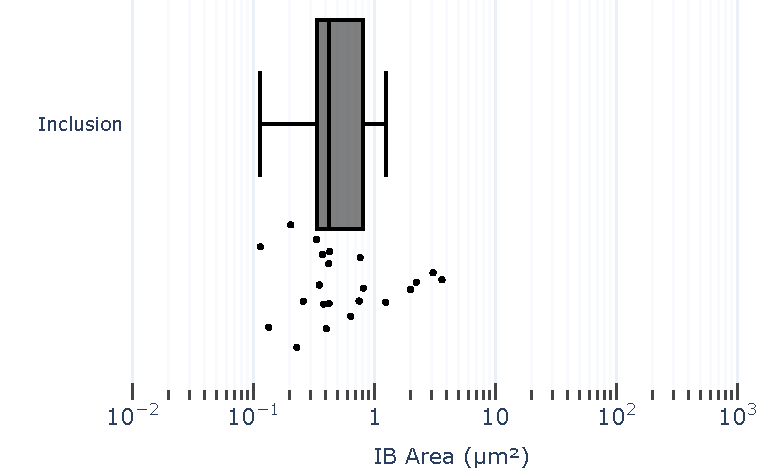
\includegraphics[width=1\linewidth]{09. Chapter 4/Figs/01. pIB/03. IFIT2/04. IFIT2-FLAG/03. FLAG/08. box_bi2f_bnbp.pdf}
    \end{subfigure}
    \caption[Observed Phenotypes of Exogenous Bovine IFIT2 in the Context of bRSV Pseudo Inclusion Bodies in Vero Cell Line, as Detected by FLAG Antibody.]{\textbf{Observed Phenotypes of Exogenous Bovine IFIT2 in the Context of bRSV Pseudo Inclusion Bodies in Vero Cell Line, as Detected by FLAG Antibody.} Vero cells were transfected with bRSV N and P, along with bovine IFIT2-FLAG containing plasmids using TransIT-X2 and were fixed after 24 hours. Cells were labeled with anti-RSV N and anti-FLAG antibodies and imaged on confocal microscope. Panel (a) shows percentual proportions of observed phenotypes between bRSV pseudo inclusion bodies and exogenous bovine IFIT2 (22 observations), with the red dotted line denoting the 5\% threshold, marking phenotypes considered relevant above this limit. Panel (b) shows the IB area in \(\mu \mbox{m}^2\) per observed relevant phenotype.}
    \label{fig:Observed Phenotypes of Exogenous Bovine IFIT2 in the Context of bRSV Pseudo Inclusion Bodies in Vero Cell Line, as Detected by FLAG Antibody}
\end{figure}

\begin{figure}
    \centering
    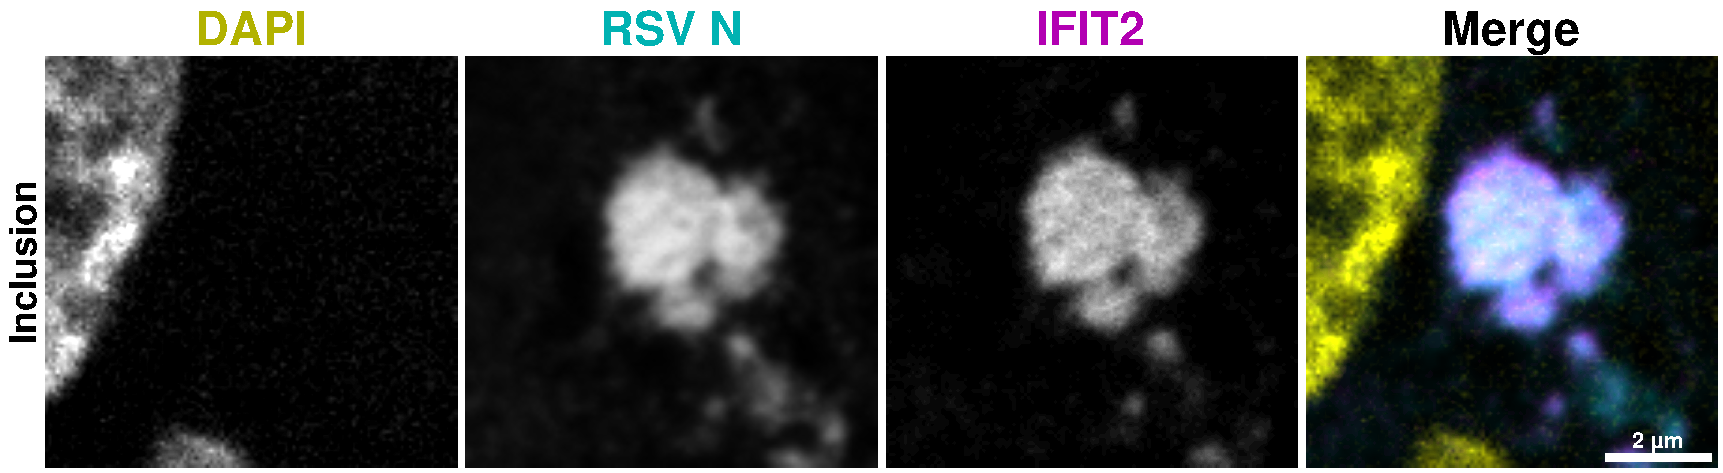
\includegraphics[width=1\linewidth]{09. Chapter 4/Figs/01. pIB/03. IFIT2/04. IFIT2-FLAG/03. FLAG/09. bi2f-bnbp.pdf}
    \caption[Representative Images of Observed Phenotypes of Exogenous Bovine IFIT2 in the Context of bRSV Pseudo Inclusion Bodies in Vero Cell Line, as Detected by FLAG Antibody.]{\textbf{Representative Images of Observed Phenotypes of Exogenous Bovine IFIT2 in the Context of bRSV Pseudo Inclusion Bodies in Vero Cell Line, as Detected by FLAG Antibody.} Vero cells were transfected with bRSV N and P, along with bovine IFIT2-FLAG containing plasmids using TransIT-X2 and were fixed after 24 hours. Cellular nuclei were stained with DAPI (yellow), and cells were double-labeled with anti-RSV N (cyan) and anti-FLAG (magenta) antibodies. This figure showcases representative examples of relevant phenotypes in the interaction between exogenous bovine IFIT2 and bRSV pseudo inclusion bodies. These phenotypes are presented in descending order based on their percentage proportions. The scale bar indicates 2 \(\mu \mbox{m}\).}
    \label{fig:Representative Images of Observed Phenotypes of Exogenous Bovine IFIT2 in the Context of bRSV Pseudo Inclusion Bodies in Vero Cell Line, as Detected by FLAG Antibody}
\end{figure}

100
0.41

%infection

\begin{figure}
    \begin{subfigure}{0.495\textwidth}
        \caption{}
        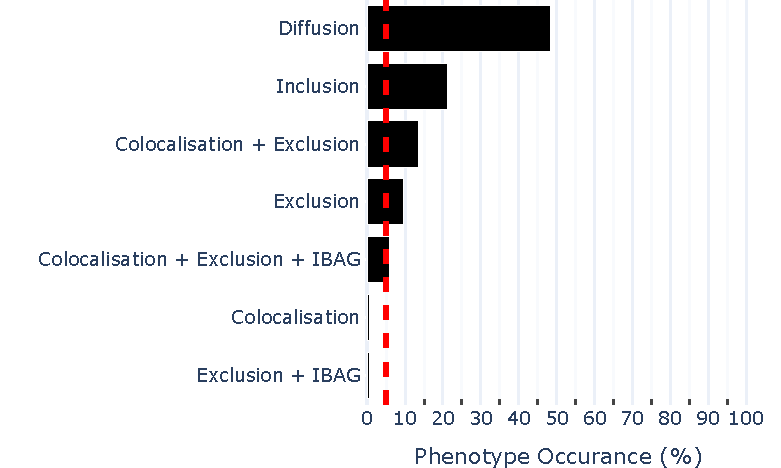
\includegraphics[width=1\linewidth]{09. Chapter 4/Figs/02. Overexpression/02. IFIT2/01. bar_hi2f_hrsv.pdf} 
    \end{subfigure}
    \begin{subfigure}{0.495\textwidth}
        \caption{}
        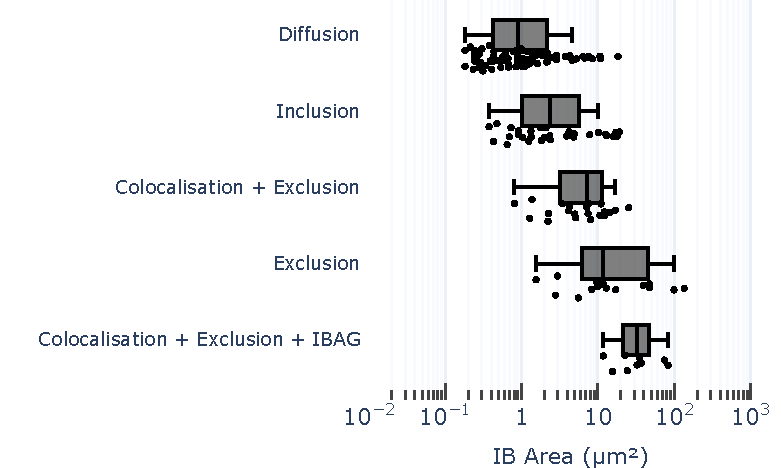
\includegraphics[width=1\linewidth]{09. Chapter 4/Figs/02. Overexpression/02. IFIT2/02. box_hi2f_hrsv.pdf}
    \end{subfigure}
    \caption[Observed Phenotypes of Exogenous hIFIT2 in the Context of hRSV Inclusion Bodies in Vero Cell Line.]{\textbf{Observed Phenotypes of Exogenous hIFIT2 in the Context of hRSV Inclusion Bodies in Vero Cell Line.} Vero cells were infected with human RSV at MOI 1. 24 HPI, the cells were transfected with hIFIT2-FLAG containing plasmids using TransIT-X2 and were fixed after further 24 hours. Cells were labeled with anti-RSV N and anti-FLAG antibodies and imaged on confocal microscope. Panel (a) shows percentual proportions of observed phenotypes between hRSV inclusion bodies and exogenous hIFIT2 (155 observations), with the red dotted line denoting the 5\% threshold, marking phenotypes considered relevant above this limit. Panel (b) shows the IB area in \(\mu \mbox{m}^2\) per observed relevant phenotype.}
    \label{fig:Observed Phenotypes of Exogenous hIFIT2 in the Context of hRSV Inclusion Bodies in Vero Cell Line}
\end{figure}

\begin{figure}
    \centering
    \includegraphics[width=1\linewidth]{09. Chapter 4/Figs/02. Overexpression/02. IFIT2/03. hi2f-hrsv.pdf}
    \caption[Representative Images of Observed Phenotypes of Exogenous hIFIT2 in the Context of hRSV Inclusion Bodies in Vero Cell Line.]{\textbf{Representative Images of Observed Phenotypes of Exogenous hIFIT2 in the Context of hRSV Inclusion Bodies in Vero Cell Line.} Vero cells were infected with human RSV at MOI 1. 24 HPI, the cells were transfected with hIFIT2-FLAG containing plasmids using TransIT-X2 and were fixed after further 24 hours. Cellular nuclei were stained with DAPI (yellow), and cells were double-labeled with anti-RSV N (cyan) and anti-FLAG (magenta) antibodies. This figure showcases representative examples of relevant phenotypes in the interaction between exogenous hIFIT2 and hRSV inclusion bodies. These phenotypes are presented in descending order based on their percentage proportions. The scale bar indicates 2 \(\mu \mbox{m}\).}
    \label{fig:Representative Images of Observed Phenotypes of Exogenous hIFIT2 in the Context of hRSV Inclusion Bodies in Vero Cell Line}
\end{figure}

48 21 14 9 5
0.9 2.1 7 11 32

In the follow up experiment, exogenous bovine IFIT2 in the context of human RSV infection shows the same two phenotypes. It is either excluded from the IBs (middle panel) or colocalises with the ring structure of the IBs (top and bottom panel; highlighted with arrows).

\begin{figure}
    \begin{subfigure}{0.495\textwidth}
        \caption{}
        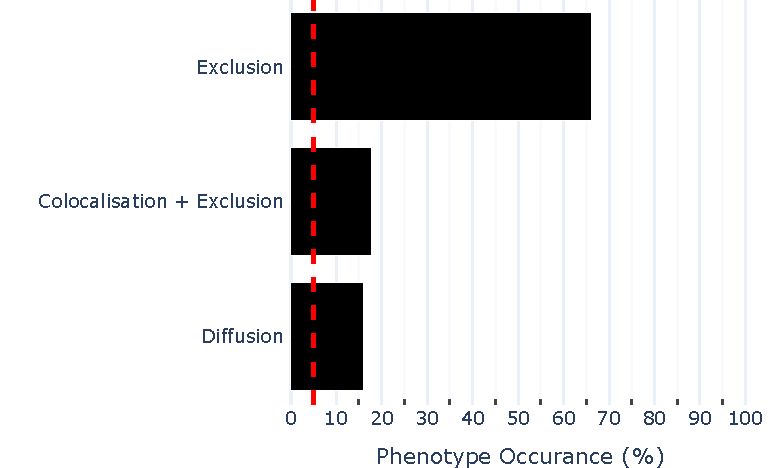
\includegraphics[width=1\linewidth]{09. Chapter 4/Figs/02. Overexpression/02. IFIT2/04. bar_bi2f_hrsv.pdf} 
    \end{subfigure}
    \begin{subfigure}{0.495\textwidth}
        \caption{}
        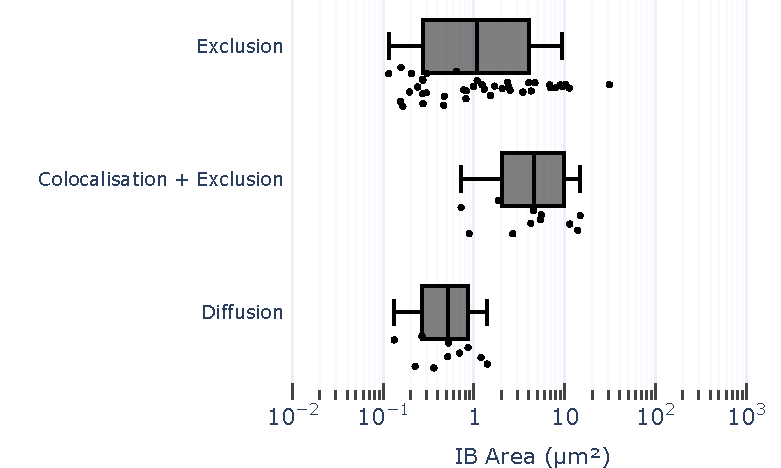
\includegraphics[width=1\linewidth]{09. Chapter 4/Figs/02. Overexpression/02. IFIT2/05. box_bi2f_hrsv.pdf}
    \end{subfigure}
    \caption[Observed Phenotypes of Exogenous bIFIT2 in the Context of hRSV Inclusion Bodies in Vero Cell Line.]{\textbf{Observed Phenotypes of Exogenous bIFIT2 in the Context of hRSV Inclusion Bodies in Vero Cell Line.} Vero cells were infected with human RSV at MOI 1. 24 HPI, the cells were transfected with bIFIT2-FLAG containing plasmids using TransIT-X2 and were fixed after further 24 hours. Cells were labeled with anti-RSV N and anti-FLAG antibodies and imaged on confocal microscope. Panel (a) shows percentual proportions of observed phenotypes between hRSV inclusion bodies and exogenous bIFIT2 (62 observations), with the red dotted line denoting the 5\% threshold, marking phenotypes considered relevant above this limit. Panel (b) shows the IB area in \(\mu \mbox{m}^2\) per observed relevant phenotype.}
    \label{fig:Observed Phenotypes of Exogenous bIFIT2 in the Context of hRSV Inclusion Bodies in Vero Cell Line}
\end{figure}

\begin{figure}
    \centering
    \includegraphics[width=1\linewidth]{09. Chapter 4/Figs/02. Overexpression/02. IFIT2/06. bi2f-hrsv.pdf}
    \caption[Representative Images of Observed Phenotypes of Exogenous bIFIT2 in the Context of hRSV Inclusion Bodies in Vero Cell Line.]{\textbf{Representative Images of Observed Phenotypes of Exogenous bIFIT2 in the Context of hRSV Inclusion Bodies in Vero Cell Line.} Vero cells were infected with human RSV at MOI 1. 24 HPI, the cells were transfected with bIFIT2-FLAG containing plasmids using TransIT-X2 and were fixed after further 24 hours. Cellular nuclei were stained with DAPI (yellow), and cells were double-labeled with anti-RSV N (cyan) and anti-FLAG (magenta) antibodies. This figure showcases representative examples of relevant phenotypes in the interaction between exogenous bIFIT2 and hRSV inclusion bodies. These phenotypes are presented in descending order based on their percentage proportions. The scale bar indicates 2 \(\mu \mbox{m}\).}
    \label{fig:Representative Images of Observed Phenotypes of Exogenous bIFIT2 in the Context of hRSV Inclusion Bodies in Vero Cell Line}
\end{figure}

66 17 16
1 5 0.5

Exogenous bovine IFIT2 during bovine RSV infection seems to be excluded from the inclusion bodies, although the data is not great and the IFIT2 is aggregated in both cells shown.

\begin{figure}
    \begin{subfigure}{0.495\textwidth}
        \caption{}
        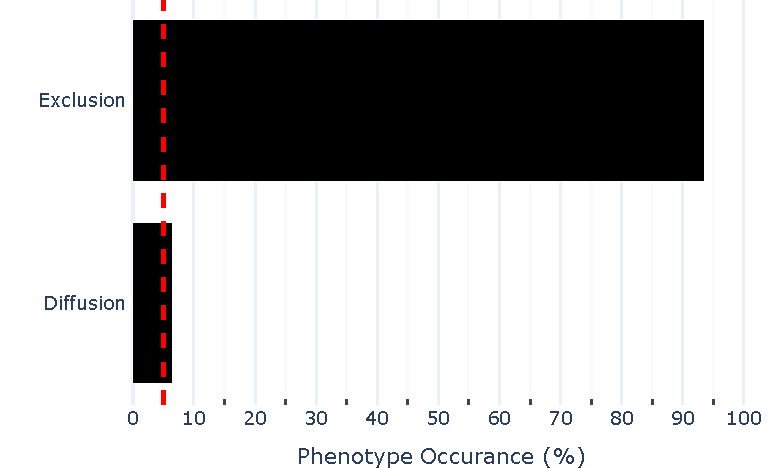
\includegraphics[width=1\linewidth]{09. Chapter 4/Figs/02. Overexpression/02. IFIT2/07. bar_bi2f_brsv.pdf} 
    \end{subfigure}
    \begin{subfigure}{0.495\textwidth}
        \caption{}
        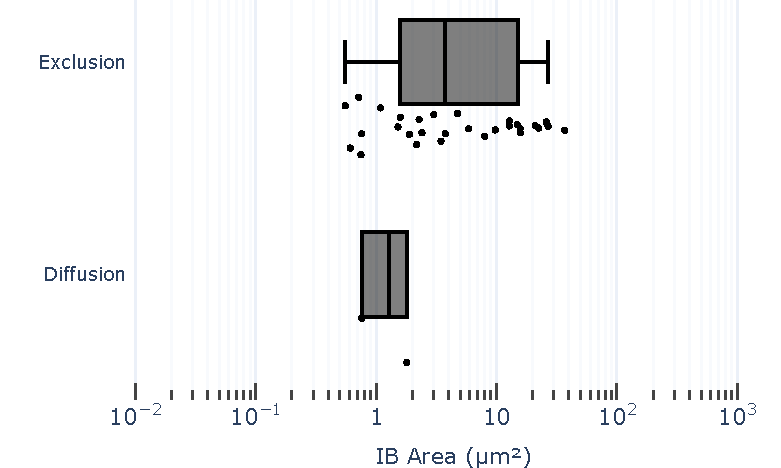
\includegraphics[width=1\linewidth]{09. Chapter 4/Figs/02. Overexpression/02. IFIT2/08. box_bi2f_brsv.pdf}
    \end{subfigure}
    \caption[Observed Phenotypes of Exogenous bIFIT2 in the Context of bRSV Inclusion Bodies in Vero Cell Line.]{\textbf{Observed Phenotypes of Exogenous bIFIT2 in the Context of bRSV Inclusion Bodies in Vero Cell Line.} Vero cells were infected with human RSV at MOI 1. 24 HPI, the cells were transfected with bIFIT2-FLAG containing plasmids using TransIT-X2 and were fixed after further 24 hours. Cells were labeled with anti-RSV N and anti-FLAG antibodies and imaged on confocal microscope. Panel (a) shows percentual proportions of observed phenotypes between bRSV inclusion bodies and exogenous bIFIT2 (31 observations), with the red dotted line denoting the 5\% threshold, marking phenotypes considered relevant above this limit. Panel (b) shows the IB area in \(\mu \mbox{m}^2\) per observed relevant phenotype.}
    \label{fig:Observed Phenotypes of Exogenous bIFIT2 in the Context of bRSV Inclusion Bodies in Vero Cell Line}
\end{figure}

\begin{figure}
    \centering
    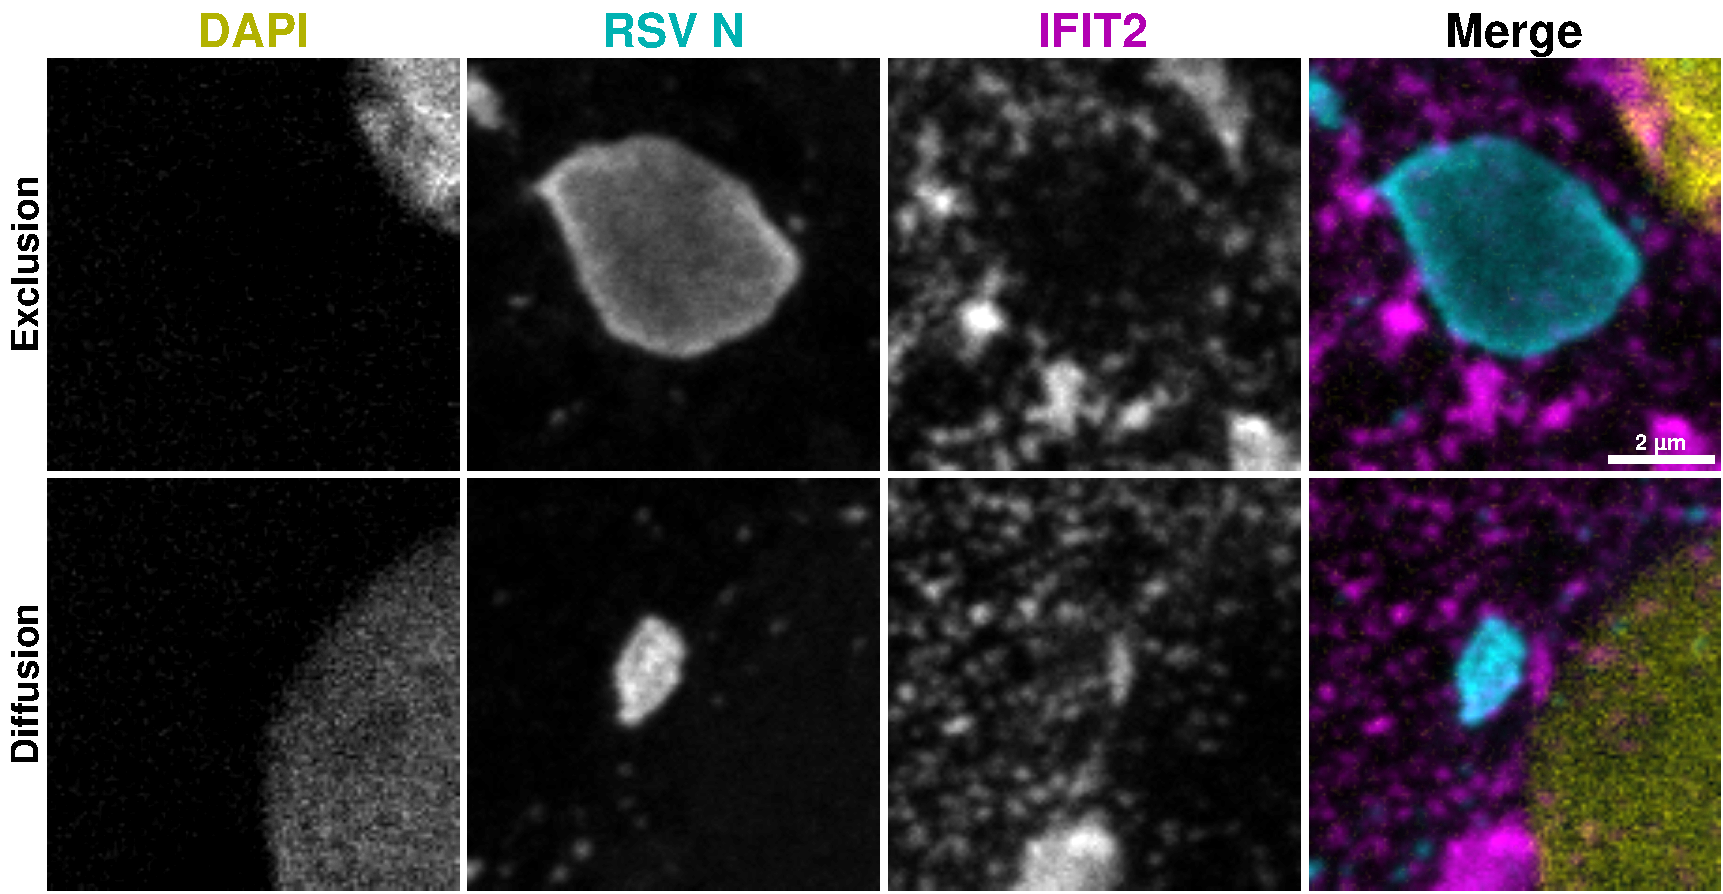
\includegraphics[width=1\linewidth]{09. Chapter 4/Figs/02. Overexpression/02. IFIT2/09. bi2f-brsv.pdf}
    \caption[Representative Images of Observed Phenotypes of Exogenous bIFIT2 in the Context of bRSV Inclusion Bodies in Vero Cell Line.]{\textbf{Representative Images of Observed Phenotypes of Exogenous bIFIT2 in the Context of bRSV Inclusion Bodies in Vero Cell Line.} Vero cells were infected with human RSV at MOI 1. 24 HPI, the cells were transfected with bIFIT2-FLAG containing plasmids using TransIT-X2 and were fixed after further 24 hours. Cellular nuclei were stained with DAPI (yellow), and cells were double-labeled with anti-RSV N (cyan) and anti-FLAG (magenta) antibodies. This figure showcases representative examples of relevant phenotypes in the interaction between exogenous bIFIT2 and bRSV inclusion bodies. These phenotypes are presented in descending order based on their percentage proportions. The scale bar indicates 2 \(\mu \mbox{m}\).}
    \label{fig:Representative Images of Observed Phenotypes of Exogenous bIFIT2 in the Context of bRSV Inclusion Bodies in Vero Cell Line}
\end{figure}

94 6
3.9 1.3

\subsection{Endeavour in Understanding the Mechanisms of IFIT2-RSV IB Interaction} \label{subsec:Endeavour in Understanding the Mechanisms of IFIT2-RSV IB Interaction}
%The Generation of Bovine IFIT2 RNA-Binding Mutant
Using published data about hIFIT2 rna-binding mutant

Difficulty of using alpha-fold with IFIT2 due to the swap domain

Using SWISS-MODEL to predict bIFIT2 structure from published hIFIT2 structures

Alignment of both structures, assessment of electrostatic charges and establishment of residues to be mutated

Primer design and mutagenesis procedure based on published hIFIT2 RNA-binding mutant paper
\cite{Tran2020InfluenzaMRNAs}

\ref{subsec:PCR for Point Mutant Generation}

\begin{figure}
    \centering
    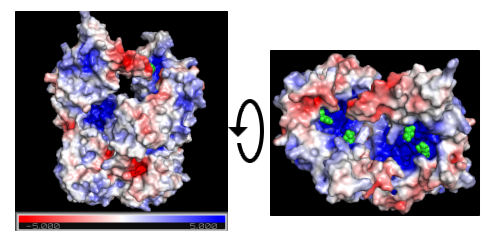
\includegraphics[width=1\linewidth]{09. Chapter 4/Figs/01. pIB/03. IFIT2/05. IFIT2-RNA binding mutant/01. Structure/01. structure.png}
    \caption[ifit2 mutant structure]{\textbf{bifit2 mutant structure.} write caption}
    \label{fig:ifit2 mutant structure}
\end{figure}


\begin{figure}
    \begin{subfigure}{0.495\textwidth}
        \caption{}
        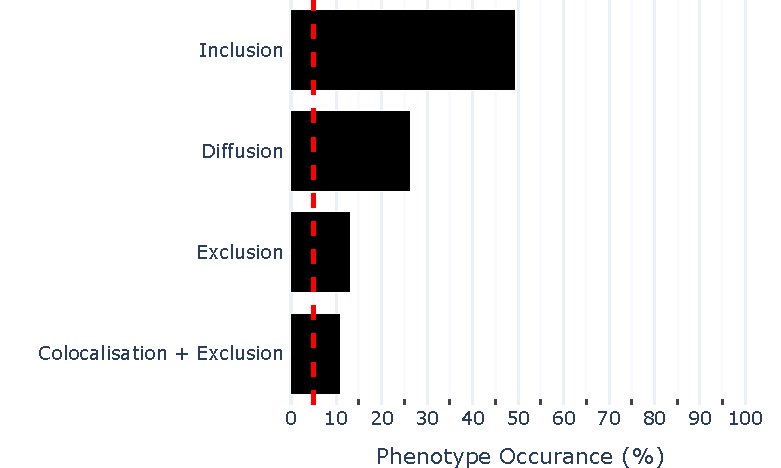
\includegraphics[width=1\linewidth]{09. Chapter 4/Figs/01. pIB/03. IFIT2/05. IFIT2-RNA binding mutant/02. pIB/01. bar_bi2f24_hnhp.pdf} 
    \end{subfigure}
    \begin{subfigure}{0.495\textwidth}
        \caption{}
        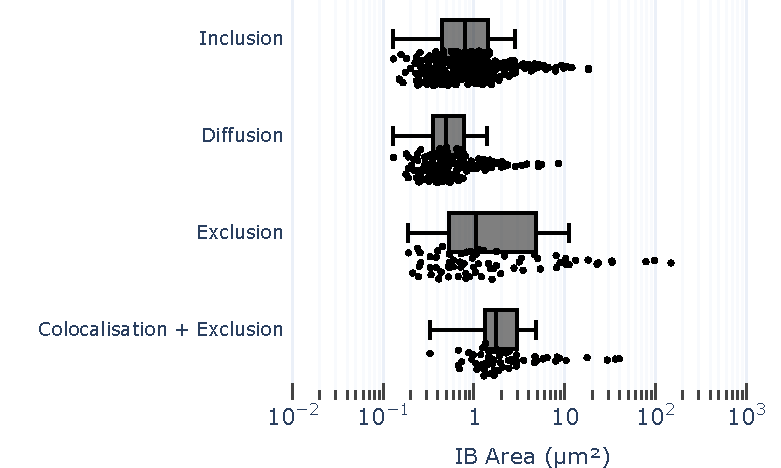
\includegraphics[width=1\linewidth]{09. Chapter 4/Figs/01. pIB/03. IFIT2/05. IFIT2-RNA binding mutant/02. pIB/02. box_bi2f24_hnhp.pdf}
    \end{subfigure}
    \caption[Diverse Phenotypic Interactions of Bovine IFIT2 RNA-Binding Mutant with Human RSV Pseudo Inclusion Bodies (pIBs) in the Vero Cell Line.]{\textbf{Diverse Phenotypic Interactions of Bovine IFIT2 RNA-Binding Mutant with Human RSV Pseudo Inclusion Bodies (pIBs) in the Vero Cell Line.} Vero cells were transfected with hRSV N and P, along with bovine IFIT2-FLAG RNA-binding mutant containing plasmids using TransIT-X2 and were fixed after 24 hours. Cells were labelled with anti-RSV N and anti-FLAG antibodies and imaged on a confocal microscope. Panel (a) shows percentual proportions of observed phenotypes between hRSV pseudo inclusion bodies and exogenous bovine IFIT2-FLAG RNA-binding mutant (548 observations), with the red dotted line denoting the 5\% threshold, marking phenotypes considered relevant above this limit. Panel (b) shows the IB area in \(\mu \mbox{m}^2\) per observed relevant phenotype.}
    \label{fig:Diverse Phenotypic Interactions of Bovine IFIT2 RNA-Binding Mutant with Human RSV Pseudo Inclusion Bodies (pIBs) in the Vero Cell Line}
\end{figure}

\begin{figure}
    \centering
    \includegraphics[width=1\linewidth]{09. Chapter 4/Figs/01. pIB/03. IFIT2/05. IFIT2-RNA binding mutant/02. pIB/03. bi2f24-hnhp.pdf}
    \caption[Representative Images of Diverse Phenotypic Interactions of Bovine IFIT2 RNA-Binding Mutant with Human RSV Pseudo Inclusion Bodies (pIBs) in the Vero Cell Line.]{\textbf{Representative Images of Diverse Phenotypic Interactions of Bovine IFIT2 RNA-Binding Mutant with Human RSV Pseudo Inclusion Bodies (pIBs) in the Vero Cell Line.}  Vero cells were transfected with bRSV N and P, along with bovine IFIT2-FLAG RNA-binding mutant containing plasmids using TransIT-X2 and were fixed after 24 hours. Cellular nuclei were stained with DAPI (yellow), and cells were double-labelled with anti-RSV N (cyan) and anti-FLAG (magenta) antibodies. This figure showcases representative examples of relevant phenotypes in the interaction between exogenous bovine IFIT2-FLAG RNA-binding mutant and hRSV pseudo inclusion bodies. These phenotypes are presented in descending order based on their percentage proportions. The scale bar indicates 2 \(\mu \mbox{m}\).}
    \label{fig:Representative Images of Diverse Phenotypic Interactions of Bovine IFIT2 RNA-Binding Mutant with Human RSV Pseudo Inclusion Bodies (pIBs) in the Vero Cell Line}
\end{figure}

49 27 13 11
0.8 0.5 1 1.8

\begin{figure}
    \begin{subfigure}{0.495\textwidth}
        \caption{}
        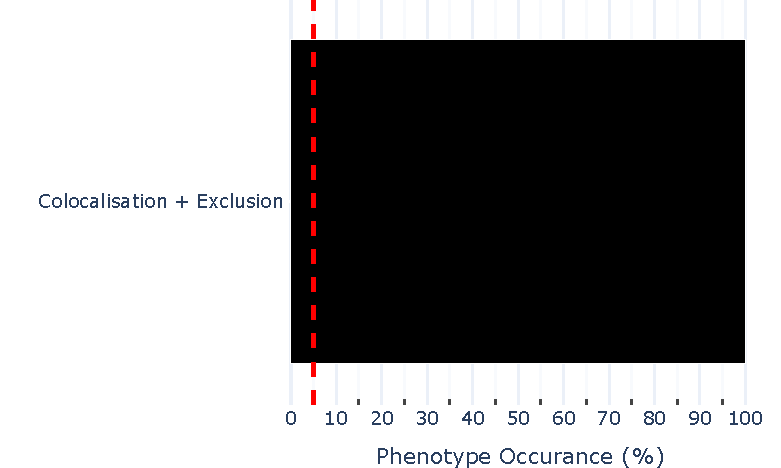
\includegraphics[width=1\linewidth]{09. Chapter 4/Figs/01. pIB/03. IFIT2/05. IFIT2-RNA binding mutant/02. pIB/04. bar_bi2f24_bnbp.pdf} 
    \end{subfigure}
    \begin{subfigure}{0.495\textwidth}
        \caption{}
        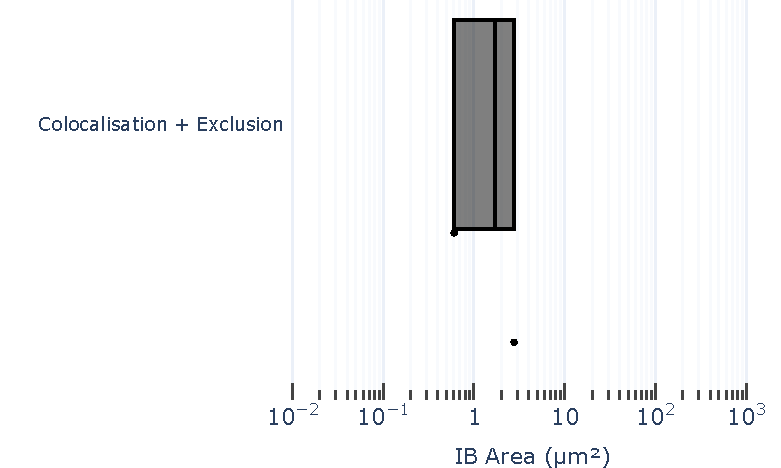
\includegraphics[width=1\linewidth]{09. Chapter 4/Figs/01. pIB/03. IFIT2/05. IFIT2-RNA binding mutant/02. pIB/05. box_bi2f24_bnbp.pdf}
    \end{subfigure}
    \caption[Diverse Phenotypic Interactions of Bovine IFIT2 RNA-Binding Mutant with Bovine RSV Pseudo Inclusion Bodies (pIBs) in the Vero Cell Line.]{\textbf{Diverse Phenotypic Interactions of Bovine IFIT2 RNA-Binding Mutant with Bovine RSV Pseudo Inclusion Bodies (pIBs) in the Vero Cell Line.} Vero cells were transfected with bRSV N and P, along with bovine IFIT2-FLAG RNA-binding mutant containing plasmids using TransIT-X2 and were fixed after 24 hours. Cells were labelled with anti-RSV N and anti-FLAG antibodies and imaged on a confocal microscope. Panel (a) shows percentual proportions of observed phenotypes between bRSV pseudo inclusion bodies and exogenous bovine IFIT2-FLAG RNA-binding mutant (2 observations), with the red dotted line denoting the 5\% threshold, marking phenotypes considered relevant above this limit. Panel (b) shows the IB area in \(\mu \mbox{m}^2\) per observed relevant phenotype.}
    \label{fig:Diverse Phenotypic Interactions of Bovine IFIT2 RNA-Binding Mutant with Bovine RSV Pseudo Inclusion Bodies (pIBs) in the Vero Cell Line}
\end{figure}

\begin{figure}
    \centering
    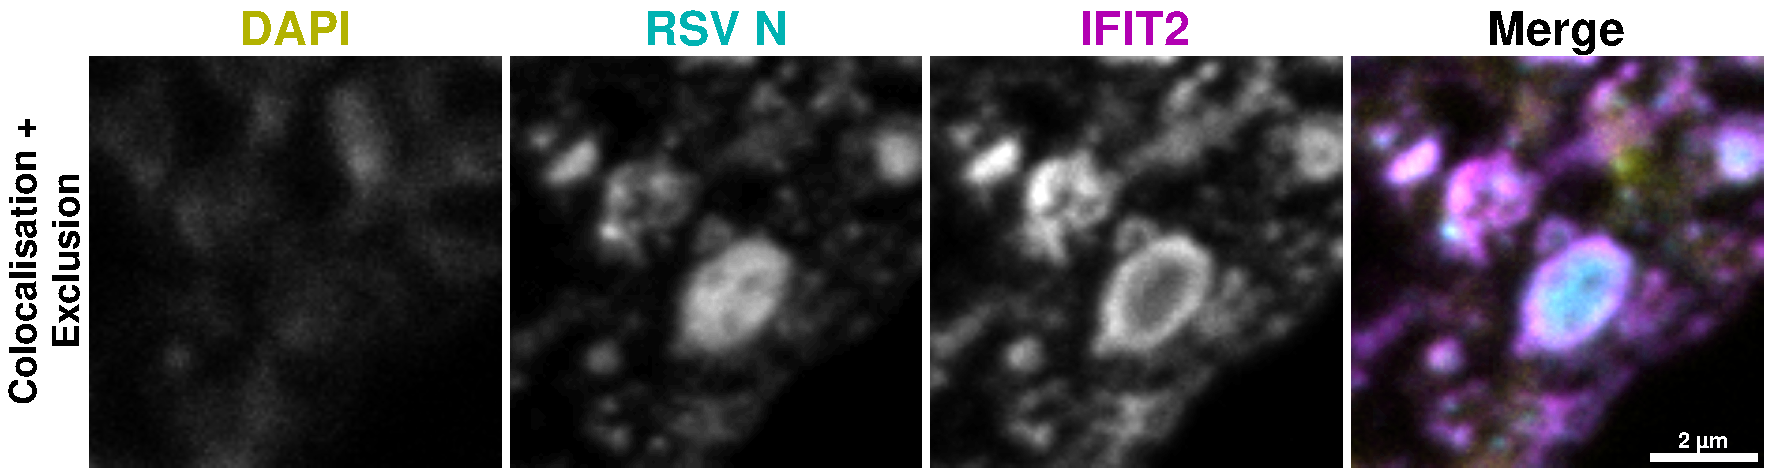
\includegraphics[width=1\linewidth]{09. Chapter 4/Figs/01. pIB/03. IFIT2/05. IFIT2-RNA binding mutant/02. pIB/06. bi2f24-bnbp.pdf}
    \caption[Representative Images of Diverse Phenotypic Interactions of Bovine IFIT2 RNA-Binding Mutant with Bovine RSV Pseudo Inclusion Bodies (pIBs) in the Vero Cell Line.]{\textbf{Representative Images of Diverse Phenotypic Interactions of Bovine IFIT2 RNA-Binding Mutant with Bovine RSV Pseudo Inclusion Bodies (pIBs) in the Vero Cell Line.}  Vero cells were transfected with bRSV N and P, along with bovine IFIT2-FLAG RNA-binding mutant containing plasmids using TransIT-X2 and were fixed after 24 hours. Cellular nuclei were stained with DAPI (yellow), and cells were double-labelled with anti-RSV N (cyan) and anti-FLAG (magenta) antibodies. This figure showcases representative examples of relevant phenotypes in the interaction between exogenous bovine IFIT2-FLAG RNA-binding mutant and bRSV pseudo inclusion bodies. These phenotypes are presented in descending order based on their percentage proportions. The scale bar indicates 2 \(\mu \mbox{m}\).}
    \label{fig:Representative Images of Diverse Phenotypic Interactions of Bovine IFIT2 RNA-Binding Mutant with Bovine RSV Pseudo Inclusion Bodies (pIBs) in the Vero Cell Line}
\end{figure}

100
1.8

% summary i2
We have described how bovine IFIT2 RNA-binding mutant was designed based on the published human IFIT2 RNA-binding mutant data (needs to be annotated more). Overexpression of bovine IFIT2 RNA-binding mutant yields cellular distribution and morphology similar to what was observed with overexpressing human IFIT2-FLAG, suggesting that the mutant proteins are not toxic to the cells. In the first experiment where we were looking at interaction between bovine IFIT2 RNA-binding mutant and human pseudo inclusion bodies we saw several phenotypes. We observed bovine IFIT2 RNA-binding mutant being excluded from small and big pIBs and pIB associated filamentous network, while fully or partially colocalising with other pIBs. In a subsequent experiment we observed only colocalization and inclusion formation. When assessing the interaction between bovine IFIT2 RNA-binding mutant and human pIBs formed using wild-type human RSV P and GFP-tagged human RSV N, we observed consistently in two experiments that bovine IFIT2 RNA-binding mutant colocalises to the pIB structures.